\documentclass[twoside]{book}

% Packages required by doxygen
\usepackage{fixltx2e}
\usepackage{calc}
\usepackage{doxygen}
\usepackage[export]{adjustbox} % also loads graphicx
\usepackage{graphicx}
\usepackage[utf8]{inputenc}
\usepackage{makeidx}
\usepackage{multicol}
\usepackage{multirow}
\PassOptionsToPackage{warn}{textcomp}
\usepackage{textcomp}
\usepackage[nointegrals]{wasysym}
\usepackage[table]{xcolor}

% Font selection
\usepackage[T1]{fontenc}
\usepackage[scaled=.90]{helvet}
\usepackage{courier}
\usepackage{amssymb}
\usepackage{sectsty}
\renewcommand{\familydefault}{\sfdefault}
\allsectionsfont{%
  \fontseries{bc}\selectfont%
  \color{darkgray}%
}
\renewcommand{\DoxyLabelFont}{%
  \fontseries{bc}\selectfont%
  \color{darkgray}%
}
\newcommand{\+}{\discretionary{\mbox{\scriptsize$\hookleftarrow$}}{}{}}

% Page & text layout
\usepackage{geometry}
\geometry{%
  a4paper,%
  top=2.5cm,%
  bottom=2.5cm,%
  left=2.5cm,%
  right=2.5cm%
}
\tolerance=750
\hfuzz=15pt
\hbadness=750
\setlength{\emergencystretch}{15pt}
\setlength{\parindent}{0cm}
\setlength{\parskip}{3ex plus 2ex minus 2ex}
\makeatletter
\renewcommand{\paragraph}{%
  \@startsection{paragraph}{4}{0ex}{-1.0ex}{1.0ex}{%
    \normalfont\normalsize\bfseries\SS@parafont%
  }%
}
\renewcommand{\subparagraph}{%
  \@startsection{subparagraph}{5}{0ex}{-1.0ex}{1.0ex}{%
    \normalfont\normalsize\bfseries\SS@subparafont%
  }%
}
\makeatother

% Headers & footers
\usepackage{fancyhdr}
\pagestyle{fancyplain}
\fancyhead[LE]{\fancyplain{}{\bfseries\thepage}}
\fancyhead[CE]{\fancyplain{}{}}
\fancyhead[RE]{\fancyplain{}{\bfseries\leftmark}}
\fancyhead[LO]{\fancyplain{}{\bfseries\rightmark}}
\fancyhead[CO]{\fancyplain{}{}}
\fancyhead[RO]{\fancyplain{}{\bfseries\thepage}}
\fancyfoot[LE]{\fancyplain{}{}}
\fancyfoot[CE]{\fancyplain{}{}}
\fancyfoot[RE]{\fancyplain{}{\bfseries\scriptsize Generated by Doxygen }}
\fancyfoot[LO]{\fancyplain{}{\bfseries\scriptsize Generated by Doxygen }}
\fancyfoot[CO]{\fancyplain{}{}}
\fancyfoot[RO]{\fancyplain{}{}}
\renewcommand{\footrulewidth}{0.4pt}
\renewcommand{\chaptermark}[1]{%
  \markboth{#1}{}%
}
\renewcommand{\sectionmark}[1]{%
  \markright{\thesection\ #1}%
}

% Indices & bibliography
\usepackage{natbib}
\usepackage[titles]{tocloft}
\setcounter{tocdepth}{3}
\setcounter{secnumdepth}{5}
\makeindex

% Hyperlinks (required, but should be loaded last)
\usepackage{ifpdf}
\ifpdf
  \usepackage[pdftex,pagebackref=true]{hyperref}
\else
  \usepackage[ps2pdf,pagebackref=true]{hyperref}
\fi
\hypersetup{%
  colorlinks=true,%
  linkcolor=blue,%
  citecolor=blue,%
  unicode%
}

% Custom commands
\newcommand{\clearemptydoublepage}{%
  \newpage{\pagestyle{empty}\cleardoublepage}%
}

\usepackage{caption}
\captionsetup{labelsep=space,justification=centering,font={bf},singlelinecheck=off,skip=4pt,position=top}

%===== C O N T E N T S =====

\begin{document}

% Titlepage & ToC
\hypersetup{pageanchor=false,
             bookmarksnumbered=true,
             pdfencoding=unicode
            }
\pagenumbering{alph}
\begin{titlepage}
\vspace*{7cm}
\begin{center}%
{\Large Neurio \\[1ex]\large 0.\+01 }\\
\vspace*{1cm}
{\large Generated by Doxygen 1.8.13}\\
\end{center}
\end{titlepage}
\clearemptydoublepage
\pagenumbering{roman}
\tableofcontents
\clearemptydoublepage
\pagenumbering{arabic}
\hypersetup{pageanchor=true}

%--- Begin generated contents ---
\chapter{Namespace Index}
\section{Packages}
Here are the packages with brief descriptions (if available)\+:\begin{DoxyCompactList}
\item\contentsline{section}{\hyperlink{namespaceneur_i_o}{neur\+IO} }{\pageref{namespaceneur_i_o}}{}
\item\contentsline{section}{\hyperlink{namespaceneur_i_o_1_1data}{neur\+I\+O.\+data} }{\pageref{namespaceneur_i_o_1_1data}}{}
\item\contentsline{section}{\hyperlink{namespaceneur_i_o_1_1data_1_1bit_input}{neur\+I\+O.\+data.\+bit\+Input} }{\pageref{namespaceneur_i_o_1_1data_1_1bit_input}}{}
\item\contentsline{section}{\hyperlink{namespaceneur_i_o_1_1engine}{neur\+I\+O.\+engine} }{\pageref{namespaceneur_i_o_1_1engine}}{}
\item\contentsline{section}{\hyperlink{namespaceneur_i_o_1_1gui}{neur\+I\+O.\+gui} }{\pageref{namespaceneur_i_o_1_1gui}}{}
\item\contentsline{section}{\hyperlink{namespaceneur_i_o_1_1system}{neur\+I\+O.\+system} }{\pageref{namespaceneur_i_o_1_1system}}{}
\end{DoxyCompactList}

\chapter{Hierarchical Index}
\section{Class Hierarchy}
This inheritance list is sorted roughly, but not completely, alphabetically\+:\begin{DoxyCompactList}
\item \contentsline{section}{neur\+I\+O.\+data.\+bit\+Input.\+Bit\+Input\+Set}{\pageref{classneur_i_o_1_1data_1_1bit_input_1_1_bit_input_set}}{}
\item \contentsline{section}{neur\+I\+O.\+data.\+Bit\+Pagenator}{\pageref{classneur_i_o_1_1data_1_1_bit_pagenator}}{}
\item \contentsline{section}{neur\+I\+O.\+data.\+Bit\+Set}{\pageref{classneur_i_o_1_1data_1_1_bit_set}}{}
\item \contentsline{section}{neur\+I\+O.\+engine.\+Column}{\pageref{classneur_i_o_1_1engine_1_1_column}}{}
\item \contentsline{section}{neur\+I\+O.\+Global}{\pageref{classneur_i_o_1_1_global}}{}
\item \contentsline{section}{main\+Win}{\pageref{classmain_win}}{}
\item \contentsline{section}{neur\+I\+O.\+gui.\+main\+Win}{\pageref{classneur_i_o_1_1gui_1_1main_win}}{}
\item \contentsline{section}{neur\+I\+O.\+engine.\+Network}{\pageref{classneur_i_o_1_1engine_1_1_network}}{}
\item \contentsline{section}{neur\+I\+O.\+system.\+Node}{\pageref{classneur_i_o_1_1system_1_1_node}}{}
\begin{DoxyCompactList}
\item \contentsline{section}{neur\+I\+O.\+data.\+bit\+Input.\+Bit\+Input}{\pageref{classneur_i_o_1_1data_1_1bit_input_1_1_bit_input}}{}
\item \contentsline{section}{neur\+I\+O.\+system.\+Neuron}{\pageref{classneur_i_o_1_1system_1_1_neuron}}{}
\item \contentsline{section}{neur\+I\+O.\+system.\+Output\+Node}{\pageref{classneur_i_o_1_1system_1_1_output_node}}{}
\end{DoxyCompactList}
\item \contentsline{section}{neur\+I\+O.\+Start}{\pageref{classneur_i_o_1_1_start}}{}
\item \contentsline{section}{neur\+I\+O.\+system.\+Truth}{\pageref{classneur_i_o_1_1system_1_1_truth}}{}
\item \contentsline{section}{neur\+I\+O.\+system.\+Truth\+Table}{\pageref{classneur_i_o_1_1system_1_1_truth_table}}{}
\end{DoxyCompactList}

\chapter{Class Index}
\section{Class List}
Here are the classes, structs, unions and interfaces with brief descriptions\+:\begin{DoxyCompactList}
\item\contentsline{section}{\hyperlink{classneur_i_o_1_1data_1_1bit_input_1_1_bit_input}{neur\+I\+O.\+data.\+bit\+Input.\+Bit\+Input} }{\pageref{classneur_i_o_1_1data_1_1bit_input_1_1_bit_input}}{}
\item\contentsline{section}{\hyperlink{classneur_i_o_1_1data_1_1bit_input_1_1_bit_input_set}{neur\+I\+O.\+data.\+bit\+Input.\+Bit\+Input\+Set} }{\pageref{classneur_i_o_1_1data_1_1bit_input_1_1_bit_input_set}}{}
\item\contentsline{section}{\hyperlink{classneur_i_o_1_1data_1_1_bit_pagenator}{neur\+I\+O.\+data.\+Bit\+Pagenator} }{\pageref{classneur_i_o_1_1data_1_1_bit_pagenator}}{}
\item\contentsline{section}{\hyperlink{classneur_i_o_1_1data_1_1_bit_set}{neur\+I\+O.\+data.\+Bit\+Set} }{\pageref{classneur_i_o_1_1data_1_1_bit_set}}{}
\item\contentsline{section}{\hyperlink{classneur_i_o_1_1engine_1_1_column}{neur\+I\+O.\+engine.\+Column} }{\pageref{classneur_i_o_1_1engine_1_1_column}}{}
\item\contentsline{section}{\hyperlink{classneur_i_o_1_1_global}{neur\+I\+O.\+Global} }{\pageref{classneur_i_o_1_1_global}}{}
\item\contentsline{section}{\hyperlink{classmain_win}{main\+Win} }{\pageref{classmain_win}}{}
\item\contentsline{section}{\hyperlink{classneur_i_o_1_1gui_1_1main_win}{neur\+I\+O.\+gui.\+main\+Win} }{\pageref{classneur_i_o_1_1gui_1_1main_win}}{}
\item\contentsline{section}{\hyperlink{classneur_i_o_1_1engine_1_1_network}{neur\+I\+O.\+engine.\+Network} }{\pageref{classneur_i_o_1_1engine_1_1_network}}{}
\item\contentsline{section}{\hyperlink{classneur_i_o_1_1system_1_1_neuron}{neur\+I\+O.\+system.\+Neuron} }{\pageref{classneur_i_o_1_1system_1_1_neuron}}{}
\item\contentsline{section}{\hyperlink{classneur_i_o_1_1system_1_1_node}{neur\+I\+O.\+system.\+Node} }{\pageref{classneur_i_o_1_1system_1_1_node}}{}
\item\contentsline{section}{\hyperlink{classneur_i_o_1_1system_1_1_output_node}{neur\+I\+O.\+system.\+Output\+Node} }{\pageref{classneur_i_o_1_1system_1_1_output_node}}{}
\item\contentsline{section}{\hyperlink{classneur_i_o_1_1_start}{neur\+I\+O.\+Start} }{\pageref{classneur_i_o_1_1_start}}{}
\item\contentsline{section}{\hyperlink{classneur_i_o_1_1system_1_1_truth}{neur\+I\+O.\+system.\+Truth} }{\pageref{classneur_i_o_1_1system_1_1_truth}}{}
\item\contentsline{section}{\hyperlink{classneur_i_o_1_1system_1_1_truth_table}{neur\+I\+O.\+system.\+Truth\+Table} }{\pageref{classneur_i_o_1_1system_1_1_truth_table}}{}
\end{DoxyCompactList}

\chapter{File Index}
\section{File List}
Here is a list of all files with brief descriptions\+:\begin{DoxyCompactList}
\item\contentsline{section}{src/\hyperlink{main_win_8java}{main\+Win.\+java} }{\pageref{main_win_8java}}{}
\item\contentsline{section}{src/neur\+I\+O/\hyperlink{_global_8java}{Global.\+java} }{\pageref{_global_8java}}{}
\item\contentsline{section}{src/neur\+I\+O/\hyperlink{_start_8java}{Start.\+java} }{\pageref{_start_8java}}{}
\item\contentsline{section}{src/neur\+I\+O/data/\hyperlink{_bit_pagenator_8java}{Bit\+Pagenator.\+java} }{\pageref{_bit_pagenator_8java}}{}
\item\contentsline{section}{src/neur\+I\+O/data/\hyperlink{_bit_set_8java}{Bit\+Set.\+java} }{\pageref{_bit_set_8java}}{}
\item\contentsline{section}{src/neur\+I\+O/data/bit\+Input/\hyperlink{_bit_input_8java}{Bit\+Input.\+java} }{\pageref{_bit_input_8java}}{}
\item\contentsline{section}{src/neur\+I\+O/data/bit\+Input/\hyperlink{_bit_input_set_8java}{Bit\+Input\+Set.\+java} }{\pageref{_bit_input_set_8java}}{}
\item\contentsline{section}{src/neur\+I\+O/engine/\hyperlink{_column_8java}{Column.\+java} }{\pageref{_column_8java}}{}
\item\contentsline{section}{src/neur\+I\+O/engine/\hyperlink{_network_8java}{Network.\+java} }{\pageref{_network_8java}}{}
\item\contentsline{section}{src/neur\+I\+O/gui/\hyperlink{neur_i_o_2gui_2main_win_8java}{main\+Win.\+java} }{\pageref{neur_i_o_2gui_2main_win_8java}}{}
\item\contentsline{section}{src/neur\+I\+O/system/\hyperlink{_neuron_8java}{Neuron.\+java} }{\pageref{_neuron_8java}}{}
\item\contentsline{section}{src/neur\+I\+O/system/\hyperlink{_node_8java}{Node.\+java} }{\pageref{_node_8java}}{}
\item\contentsline{section}{src/neur\+I\+O/system/\hyperlink{_output_node_8java}{Output\+Node.\+java} }{\pageref{_output_node_8java}}{}
\item\contentsline{section}{src/neur\+I\+O/system/\hyperlink{_truth_8java}{Truth.\+java} }{\pageref{_truth_8java}}{}
\item\contentsline{section}{src/neur\+I\+O/system/\hyperlink{_truth_table_8java}{Truth\+Table.\+java} }{\pageref{_truth_table_8java}}{}
\end{DoxyCompactList}

\chapter{Namespace Documentation}
\hypertarget{namespaceneur_i_o}{}\section{Package neur\+IO}
\label{namespaceneur_i_o}\index{neur\+IO@{neur\+IO}}
\subsection*{Packages}
\begin{DoxyCompactItemize}
\item 
package \hyperlink{namespaceneur_i_o_1_1data}{data}
\item 
package \hyperlink{namespaceneur_i_o_1_1engine}{engine}
\item 
package \hyperlink{namespaceneur_i_o_1_1gui}{gui}
\item 
package \hyperlink{namespaceneur_i_o_1_1system}{system}
\end{DoxyCompactItemize}
\subsection*{Classes}
\begin{DoxyCompactItemize}
\item 
class \hyperlink{classneur_i_o_1_1_global}{Global}
\item 
class \hyperlink{classneur_i_o_1_1_start}{Start}
\end{DoxyCompactItemize}

\hypertarget{namespaceneur_i_o_1_1data}{}\section{Package neur\+I\+O.\+data}
\label{namespaceneur_i_o_1_1data}\index{neur\+I\+O.\+data@{neur\+I\+O.\+data}}
\subsection*{Packages}
\begin{DoxyCompactItemize}
\item 
package \hyperlink{namespaceneur_i_o_1_1data_1_1bit_input}{bit\+Input}
\end{DoxyCompactItemize}
\subsection*{Classes}
\begin{DoxyCompactItemize}
\item 
class \hyperlink{classneur_i_o_1_1data_1_1_bit_pagenator}{Bit\+Pagenator}
\item 
class \hyperlink{classneur_i_o_1_1data_1_1_bit_set}{Bit\+Set}
\end{DoxyCompactItemize}

\hypertarget{namespaceneur_i_o_1_1data_1_1bit_input}{}\section{Package neur\+I\+O.\+data.\+bit\+Input}
\label{namespaceneur_i_o_1_1data_1_1bit_input}\index{neur\+I\+O.\+data.\+bit\+Input@{neur\+I\+O.\+data.\+bit\+Input}}
\subsection*{Classes}
\begin{DoxyCompactItemize}
\item 
class \hyperlink{classneur_i_o_1_1data_1_1bit_input_1_1_bit_input}{Bit\+Input}
\item 
class \hyperlink{classneur_i_o_1_1data_1_1bit_input_1_1_bit_input_set}{Bit\+Input\+Set}
\end{DoxyCompactItemize}

\hypertarget{namespaceneur_i_o_1_1engine}{}\section{Package neur\+I\+O.\+engine}
\label{namespaceneur_i_o_1_1engine}\index{neur\+I\+O.\+engine@{neur\+I\+O.\+engine}}
\subsection*{Classes}
\begin{DoxyCompactItemize}
\item 
class \hyperlink{classneur_i_o_1_1engine_1_1_column}{Column}
\item 
class \hyperlink{classneur_i_o_1_1engine_1_1_network}{Network}
\end{DoxyCompactItemize}

\hypertarget{namespaceneur_i_o_1_1gui}{}\section{Package neur\+I\+O.\+gui}
\label{namespaceneur_i_o_1_1gui}\index{neur\+I\+O.\+gui@{neur\+I\+O.\+gui}}
\subsection*{Classes}
\begin{DoxyCompactItemize}
\item 
class \hyperlink{classneur_i_o_1_1gui_1_1main_win}{main\+Win}
\end{DoxyCompactItemize}

\hypertarget{namespaceneur_i_o_1_1system}{}\section{Package neur\+I\+O.\+system}
\label{namespaceneur_i_o_1_1system}\index{neur\+I\+O.\+system@{neur\+I\+O.\+system}}
\subsection*{Classes}
\begin{DoxyCompactItemize}
\item 
class \hyperlink{classneur_i_o_1_1system_1_1_neuron}{Neuron}
\item 
class \hyperlink{classneur_i_o_1_1system_1_1_node}{Node}
\item 
class \hyperlink{classneur_i_o_1_1system_1_1_output_node}{Output\+Node}
\item 
class \hyperlink{classneur_i_o_1_1system_1_1_truth}{Truth}
\item 
class \hyperlink{classneur_i_o_1_1system_1_1_truth_table}{Truth\+Table}
\end{DoxyCompactItemize}

\chapter{Class Documentation}
\hypertarget{classneur_i_o_1_1data_1_1bit_input_1_1_bit_input}{}\section{neur\+I\+O.\+data.\+bit\+Input.\+Bit\+Input Class Reference}
\label{classneur_i_o_1_1data_1_1bit_input_1_1_bit_input}\index{neur\+I\+O.\+data.\+bit\+Input.\+Bit\+Input@{neur\+I\+O.\+data.\+bit\+Input.\+Bit\+Input}}


Inheritance diagram for neur\+I\+O.\+data.\+bit\+Input.\+Bit\+Input\+:
% FIG 0


Collaboration diagram for neur\+I\+O.\+data.\+bit\+Input.\+Bit\+Input\+:
% FIG 1
\subsection*{Public Member Functions}
\begin{DoxyCompactItemize}
\item 
\hyperlink{classneur_i_o_1_1data_1_1bit_input_1_1_bit_input_a0cb3a5e6229418b6b2fa85184c855e32}{Bit\+Input} (boolean init)
\item 
boolean \hyperlink{classneur_i_o_1_1data_1_1bit_input_1_1_bit_input_aba6bbd1b073178133b835343a45c722e}{get} ()
\item 
void \hyperlink{classneur_i_o_1_1data_1_1bit_input_1_1_bit_input_a0fc46f4c9962c8cf8dc0387ecd61cd66}{set} (boolean \hyperlink{classneur_i_o_1_1system_1_1_node_a2c6a229d3d2cbf1b313d8797b70e487a}{value})
\end{DoxyCompactItemize}
\subsection*{Additional Inherited Members}


\subsection{Detailed Description}
\subsection*{\hyperlink{classneur_i_o_1_1data_1_1bit_input_1_1_bit_input}{Bit\+Input} }

A small extension of Node that has methods for setting the \begin{DoxySeeAlso}{See also}
\hyperlink{classneur_i_o_1_1system_1_1_node_a18dfd9e4acbf3ffbbd81870d2740254b}{Node} 
\end{DoxySeeAlso}


Definition at line 15 of file Bit\+Input.\+java.



\subsection{Constructor \& Destructor Documentation}
\mbox{\Hypertarget{classneur_i_o_1_1data_1_1bit_input_1_1_bit_input_a0cb3a5e6229418b6b2fa85184c855e32}\label{classneur_i_o_1_1data_1_1bit_input_1_1_bit_input_a0cb3a5e6229418b6b2fa85184c855e32}} 
\index{neur\+I\+O\+::data\+::bit\+Input\+::\+Bit\+Input@{neur\+I\+O\+::data\+::bit\+Input\+::\+Bit\+Input}!Bit\+Input@{Bit\+Input}}
\index{Bit\+Input@{Bit\+Input}!neur\+I\+O\+::data\+::bit\+Input\+::\+Bit\+Input@{neur\+I\+O\+::data\+::bit\+Input\+::\+Bit\+Input}}
\subsubsection{\texorpdfstring{Bit\+Input()}{BitInput()}}
{\footnotesize\ttfamily neur\+I\+O.\+data.\+bit\+Input.\+Bit\+Input.\+Bit\+Input (\begin{DoxyParamCaption}\item[{boolean}]{init }\end{DoxyParamCaption})}

Constructor.


\begin{DoxyParams}{Parameters}
{\em init} & This is the initial state \\
\hline
\end{DoxyParams}


Definition at line 22 of file Bit\+Input.\+java.



\subsection{Member Function Documentation}
\mbox{\Hypertarget{classneur_i_o_1_1data_1_1bit_input_1_1_bit_input_aba6bbd1b073178133b835343a45c722e}\label{classneur_i_o_1_1data_1_1bit_input_1_1_bit_input_aba6bbd1b073178133b835343a45c722e}} 
\index{neur\+I\+O\+::data\+::bit\+Input\+::\+Bit\+Input@{neur\+I\+O\+::data\+::bit\+Input\+::\+Bit\+Input}!get@{get}}
\index{get@{get}!neur\+I\+O\+::data\+::bit\+Input\+::\+Bit\+Input@{neur\+I\+O\+::data\+::bit\+Input\+::\+Bit\+Input}}
\subsubsection{\texorpdfstring{get()}{get()}}
{\footnotesize\ttfamily boolean neur\+I\+O.\+data.\+bit\+Input.\+Bit\+Input.\+get (\begin{DoxyParamCaption}{ }\end{DoxyParamCaption})}

Get method. 

Definition at line 29 of file Bit\+Input.\+java.

\mbox{\Hypertarget{classneur_i_o_1_1data_1_1bit_input_1_1_bit_input_a0fc46f4c9962c8cf8dc0387ecd61cd66}\label{classneur_i_o_1_1data_1_1bit_input_1_1_bit_input_a0fc46f4c9962c8cf8dc0387ecd61cd66}} 
\index{neur\+I\+O\+::data\+::bit\+Input\+::\+Bit\+Input@{neur\+I\+O\+::data\+::bit\+Input\+::\+Bit\+Input}!set@{set}}
\index{set@{set}!neur\+I\+O\+::data\+::bit\+Input\+::\+Bit\+Input@{neur\+I\+O\+::data\+::bit\+Input\+::\+Bit\+Input}}
\subsubsection{\texorpdfstring{set()}{set()}}
{\footnotesize\ttfamily void neur\+I\+O.\+data.\+bit\+Input.\+Bit\+Input.\+set (\begin{DoxyParamCaption}\item[{boolean}]{value }\end{DoxyParamCaption})}

Set method. 

Definition at line 35 of file Bit\+Input.\+java.



The documentation for this class was generated from the following file\+:\begin{DoxyCompactItemize}
\item 
src/neur\+I\+O/data/bit\+Input/\hyperlink{_bit_input_8java}{Bit\+Input.\+java}\end{DoxyCompactItemize}

\hypertarget{classneur_i_o_1_1data_1_1bit_input_1_1_bit_input_set}{}\section{neur\+I\+O.\+data.\+bit\+Input.\+Bit\+Input\+Set Class Reference}
\label{classneur_i_o_1_1data_1_1bit_input_1_1_bit_input_set}\index{neur\+I\+O.\+data.\+bit\+Input.\+Bit\+Input\+Set@{neur\+I\+O.\+data.\+bit\+Input.\+Bit\+Input\+Set}}


Collaboration diagram for neur\+I\+O.\+data.\+bit\+Input.\+Bit\+Input\+Set\+:
% FIG 0
\subsection*{Public Member Functions}
\begin{DoxyCompactItemize}
\item 
\hyperlink{classneur_i_o_1_1data_1_1bit_input_1_1_bit_input_set_ab677be938cd4f30a58140f641113e3ad}{Bit\+Input\+Set} (\hyperlink{classneur_i_o_1_1data_1_1bit_input_1_1_bit_input}{Bit\+Input}\mbox{[}$\,$\mbox{]} \hyperlink{classneur_i_o_1_1data_1_1bit_input_1_1_bit_input_set_ac9670d8e46af137a974fb229451df996}{bits})
\item 
\hyperlink{classneur_i_o_1_1data_1_1bit_input_1_1_bit_input_set_a6e620b4837378dc1421a2aae62ab329d}{Bit\+Input\+Set} (\hyperlink{classneur_i_o_1_1data_1_1bit_input_1_1_bit_input}{Bit\+Input}\mbox{[}$\,$\mbox{]} \hyperlink{classneur_i_o_1_1data_1_1bit_input_1_1_bit_input_set_ac9670d8e46af137a974fb229451df996}{bits}, String \hyperlink{classneur_i_o_1_1data_1_1bit_input_1_1_bit_input_set_ae983698847d96bf735ee7379114a0cbc}{name})
\item 
void \hyperlink{classneur_i_o_1_1data_1_1bit_input_1_1_bit_input_set_af33dc6f3bd675c235115c81ea8549ee0}{num\+To\+Input} (int in)
\end{DoxyCompactItemize}
\subsection*{Public Attributes}
\begin{DoxyCompactItemize}
\item 
\hyperlink{classneur_i_o_1_1data_1_1bit_input_1_1_bit_input}{Bit\+Input} \mbox{[}$\,$\mbox{]} \hyperlink{classneur_i_o_1_1data_1_1bit_input_1_1_bit_input_set_ac9670d8e46af137a974fb229451df996}{bits}
\item 
String \hyperlink{classneur_i_o_1_1data_1_1bit_input_1_1_bit_input_set_ae983698847d96bf735ee7379114a0cbc}{name} = \char`\"{}\char`\"{}
\end{DoxyCompactItemize}


\subsection{Detailed Description}
\subsection*{\hyperlink{classneur_i_o_1_1data_1_1bit_input_1_1_bit_input_set}{Bit\+Input\+Set} }

This is a wrapper class for the Bitset, and allows one to translate an integer to bits that the network can use. 

Definition at line 12 of file Bit\+Input\+Set.\+java.



\subsection{Constructor \& Destructor Documentation}
\mbox{\Hypertarget{classneur_i_o_1_1data_1_1bit_input_1_1_bit_input_set_ab677be938cd4f30a58140f641113e3ad}\label{classneur_i_o_1_1data_1_1bit_input_1_1_bit_input_set_ab677be938cd4f30a58140f641113e3ad}} 
\index{neur\+I\+O\+::data\+::bit\+Input\+::\+Bit\+Input\+Set@{neur\+I\+O\+::data\+::bit\+Input\+::\+Bit\+Input\+Set}!Bit\+Input\+Set@{Bit\+Input\+Set}}
\index{Bit\+Input\+Set@{Bit\+Input\+Set}!neur\+I\+O\+::data\+::bit\+Input\+::\+Bit\+Input\+Set@{neur\+I\+O\+::data\+::bit\+Input\+::\+Bit\+Input\+Set}}
\subsubsection{\texorpdfstring{Bit\+Input\+Set()}{BitInputSet()}\hspace{0.1cm}{\footnotesize\ttfamily [1/2]}}
{\footnotesize\ttfamily neur\+I\+O.\+data.\+bit\+Input.\+Bit\+Input\+Set.\+Bit\+Input\+Set (\begin{DoxyParamCaption}\item[{\hyperlink{classneur_i_o_1_1data_1_1bit_input_1_1_bit_input}{Bit\+Input} \mbox{[}$\,$\mbox{]}}]{bits }\end{DoxyParamCaption})}



Definition at line 17 of file Bit\+Input\+Set.\+java.

\mbox{\Hypertarget{classneur_i_o_1_1data_1_1bit_input_1_1_bit_input_set_a6e620b4837378dc1421a2aae62ab329d}\label{classneur_i_o_1_1data_1_1bit_input_1_1_bit_input_set_a6e620b4837378dc1421a2aae62ab329d}} 
\index{neur\+I\+O\+::data\+::bit\+Input\+::\+Bit\+Input\+Set@{neur\+I\+O\+::data\+::bit\+Input\+::\+Bit\+Input\+Set}!Bit\+Input\+Set@{Bit\+Input\+Set}}
\index{Bit\+Input\+Set@{Bit\+Input\+Set}!neur\+I\+O\+::data\+::bit\+Input\+::\+Bit\+Input\+Set@{neur\+I\+O\+::data\+::bit\+Input\+::\+Bit\+Input\+Set}}
\subsubsection{\texorpdfstring{Bit\+Input\+Set()}{BitInputSet()}\hspace{0.1cm}{\footnotesize\ttfamily [2/2]}}
{\footnotesize\ttfamily neur\+I\+O.\+data.\+bit\+Input.\+Bit\+Input\+Set.\+Bit\+Input\+Set (\begin{DoxyParamCaption}\item[{\hyperlink{classneur_i_o_1_1data_1_1bit_input_1_1_bit_input}{Bit\+Input} \mbox{[}$\,$\mbox{]}}]{bits,  }\item[{String}]{name }\end{DoxyParamCaption})}



Definition at line 21 of file Bit\+Input\+Set.\+java.



\subsection{Member Function Documentation}
\mbox{\Hypertarget{classneur_i_o_1_1data_1_1bit_input_1_1_bit_input_set_af33dc6f3bd675c235115c81ea8549ee0}\label{classneur_i_o_1_1data_1_1bit_input_1_1_bit_input_set_af33dc6f3bd675c235115c81ea8549ee0}} 
\index{neur\+I\+O\+::data\+::bit\+Input\+::\+Bit\+Input\+Set@{neur\+I\+O\+::data\+::bit\+Input\+::\+Bit\+Input\+Set}!num\+To\+Input@{num\+To\+Input}}
\index{num\+To\+Input@{num\+To\+Input}!neur\+I\+O\+::data\+::bit\+Input\+::\+Bit\+Input\+Set@{neur\+I\+O\+::data\+::bit\+Input\+::\+Bit\+Input\+Set}}
\subsubsection{\texorpdfstring{num\+To\+Input()}{numToInput()}}
{\footnotesize\ttfamily void neur\+I\+O.\+data.\+bit\+Input.\+Bit\+Input\+Set.\+num\+To\+Input (\begin{DoxyParamCaption}\item[{int}]{in }\end{DoxyParamCaption})}



Definition at line 26 of file Bit\+Input\+Set.\+java.



\subsection{Member Data Documentation}
\mbox{\Hypertarget{classneur_i_o_1_1data_1_1bit_input_1_1_bit_input_set_ac9670d8e46af137a974fb229451df996}\label{classneur_i_o_1_1data_1_1bit_input_1_1_bit_input_set_ac9670d8e46af137a974fb229451df996}} 
\index{neur\+I\+O\+::data\+::bit\+Input\+::\+Bit\+Input\+Set@{neur\+I\+O\+::data\+::bit\+Input\+::\+Bit\+Input\+Set}!bits@{bits}}
\index{bits@{bits}!neur\+I\+O\+::data\+::bit\+Input\+::\+Bit\+Input\+Set@{neur\+I\+O\+::data\+::bit\+Input\+::\+Bit\+Input\+Set}}
\subsubsection{\texorpdfstring{bits}{bits}}
{\footnotesize\ttfamily \hyperlink{classneur_i_o_1_1data_1_1bit_input_1_1_bit_input}{Bit\+Input} \mbox{[}$\,$\mbox{]} neur\+I\+O.\+data.\+bit\+Input.\+Bit\+Input\+Set.\+bits}



Definition at line 14 of file Bit\+Input\+Set.\+java.

\mbox{\Hypertarget{classneur_i_o_1_1data_1_1bit_input_1_1_bit_input_set_ae983698847d96bf735ee7379114a0cbc}\label{classneur_i_o_1_1data_1_1bit_input_1_1_bit_input_set_ae983698847d96bf735ee7379114a0cbc}} 
\index{neur\+I\+O\+::data\+::bit\+Input\+::\+Bit\+Input\+Set@{neur\+I\+O\+::data\+::bit\+Input\+::\+Bit\+Input\+Set}!name@{name}}
\index{name@{name}!neur\+I\+O\+::data\+::bit\+Input\+::\+Bit\+Input\+Set@{neur\+I\+O\+::data\+::bit\+Input\+::\+Bit\+Input\+Set}}
\subsubsection{\texorpdfstring{name}{name}}
{\footnotesize\ttfamily String neur\+I\+O.\+data.\+bit\+Input.\+Bit\+Input\+Set.\+name = \char`\"{}\char`\"{}}



Definition at line 15 of file Bit\+Input\+Set.\+java.



The documentation for this class was generated from the following file\+:\begin{DoxyCompactItemize}
\item 
src/neur\+I\+O/data/bit\+Input/\hyperlink{_bit_input_set_8java}{Bit\+Input\+Set.\+java}\end{DoxyCompactItemize}

\hypertarget{classneur_i_o_1_1data_1_1_bit_pagenator}{}\section{neur\+I\+O.\+data.\+Bit\+Pagenator Class Reference}
\label{classneur_i_o_1_1data_1_1_bit_pagenator}\index{neur\+I\+O.\+data.\+Bit\+Pagenator@{neur\+I\+O.\+data.\+Bit\+Pagenator}}
\subsection*{Public Member Functions}
\begin{DoxyCompactItemize}
\item 
\hyperlink{classneur_i_o_1_1data_1_1_bit_pagenator_a83d98001fc92aebbf5cd7d230c70ba57}{Bit\+Pagenator} (int width)
\end{DoxyCompactItemize}


\subsection{Detailed Description}


Definition at line 3 of file Bit\+Pagenator.\+java.



\subsection{Constructor \& Destructor Documentation}
\mbox{\Hypertarget{classneur_i_o_1_1data_1_1_bit_pagenator_a83d98001fc92aebbf5cd7d230c70ba57}\label{classneur_i_o_1_1data_1_1_bit_pagenator_a83d98001fc92aebbf5cd7d230c70ba57}} 
\index{neur\+I\+O\+::data\+::\+Bit\+Pagenator@{neur\+I\+O\+::data\+::\+Bit\+Pagenator}!Bit\+Pagenator@{Bit\+Pagenator}}
\index{Bit\+Pagenator@{Bit\+Pagenator}!neur\+I\+O\+::data\+::\+Bit\+Pagenator@{neur\+I\+O\+::data\+::\+Bit\+Pagenator}}
\subsubsection{\texorpdfstring{Bit\+Pagenator()}{BitPagenator()}}
{\footnotesize\ttfamily neur\+I\+O.\+data.\+Bit\+Pagenator.\+Bit\+Pagenator (\begin{DoxyParamCaption}\item[{int}]{width }\end{DoxyParamCaption})}



Definition at line 8 of file Bit\+Pagenator.\+java.



The documentation for this class was generated from the following file\+:\begin{DoxyCompactItemize}
\item 
src/neur\+I\+O/data/\hyperlink{_bit_pagenator_8java}{Bit\+Pagenator.\+java}\end{DoxyCompactItemize}

\hypertarget{classneur_i_o_1_1data_1_1_bit_set}{}\section{neur\+I\+O.\+data.\+Bit\+Set Class Reference}
\label{classneur_i_o_1_1data_1_1_bit_set}\index{neur\+I\+O.\+data.\+Bit\+Set@{neur\+I\+O.\+data.\+Bit\+Set}}
\subsection*{Public Member Functions}
\begin{DoxyCompactItemize}
\item 
\mbox{\Hypertarget{classneur_i_o_1_1data_1_1_bit_set_a425a3d991ae3bae79a20216914f0475b}\label{classneur_i_o_1_1data_1_1_bit_set_a425a3d991ae3bae79a20216914f0475b}} 
{\bfseries Bit\+Set} (int width)
\item 
\mbox{\Hypertarget{classneur_i_o_1_1data_1_1_bit_set_af6f1dfe4ce5582a89dd327305d6d8f87}\label{classneur_i_o_1_1data_1_1_bit_set_af6f1dfe4ce5582a89dd327305d6d8f87}} 
void {\bfseries reset} ()
\item 
\mbox{\Hypertarget{classneur_i_o_1_1data_1_1_bit_set_a168de8cb6d3f39583c480859cefcc4e0}\label{classneur_i_o_1_1data_1_1_bit_set_a168de8cb6d3f39583c480859cefcc4e0}} 
void {\bfseries add\+Bit} (boolean b)
\item 
\mbox{\Hypertarget{classneur_i_o_1_1data_1_1_bit_set_a2d7d9ae61ce5ec45d924b150213ada2e}\label{classneur_i_o_1_1data_1_1_bit_set_a2d7d9ae61ce5ec45d924b150213ada2e}} 
void {\bfseries add\+Byte} (byte b)
\item 
\mbox{\Hypertarget{classneur_i_o_1_1data_1_1_bit_set_a4d57df84bc520d32429e6ae8ee4b2d9f}\label{classneur_i_o_1_1data_1_1_bit_set_a4d57df84bc520d32429e6ae8ee4b2d9f}} 
boolean {\bfseries is\+Locekd} ()
\item 
\mbox{\Hypertarget{classneur_i_o_1_1data_1_1_bit_set_a92a69cf498204d16c617a76c6110a3fe}\label{classneur_i_o_1_1data_1_1_bit_set_a92a69cf498204d16c617a76c6110a3fe}} 
int {\bfseries current\+Index} ()
\end{DoxyCompactItemize}
\subsection*{Private Member Functions}
\begin{DoxyCompactItemize}
\item 
\mbox{\Hypertarget{classneur_i_o_1_1data_1_1_bit_set_a53af6540a17581388d62d6f432f5d80d}\label{classneur_i_o_1_1data_1_1_bit_set_a53af6540a17581388d62d6f432f5d80d}} 
void {\bfseries set\+Lock} ()
\end{DoxyCompactItemize}
\subsection*{Static Private Attributes}
\begin{DoxyCompactItemize}
\item 
\mbox{\Hypertarget{classneur_i_o_1_1data_1_1_bit_set_a65b3856567b2b7fee83193e320fe11e2}\label{classneur_i_o_1_1data_1_1_bit_set_a65b3856567b2b7fee83193e320fe11e2}} 
static final long {\bfseries serial\+Version\+U\+ID} = -\/8960459244413913816L
\end{DoxyCompactItemize}


The documentation for this class was generated from the following file\+:\begin{DoxyCompactItemize}
\item 
Neur\+I\+O/src/neur\+I\+O/data/Bit\+Set.\+java\end{DoxyCompactItemize}

\hypertarget{classneur_i_o_1_1engine_1_1_column}{}\section{neur\+I\+O.\+engine.\+Column Class Reference}
\label{classneur_i_o_1_1engine_1_1_column}\index{neur\+I\+O.\+engine.\+Column@{neur\+I\+O.\+engine.\+Column}}
\subsection*{Public Member Functions}
\begin{DoxyCompactItemize}
\item 
\mbox{\Hypertarget{classneur_i_o_1_1engine_1_1_column_a5c50cb359c8494adc1d3a240131ac6bd}\label{classneur_i_o_1_1engine_1_1_column_a5c50cb359c8494adc1d3a240131ac6bd}} 
{\bfseries Column} (Node... nodes)
\item 
\mbox{\Hypertarget{classneur_i_o_1_1engine_1_1_column_a19d03fcb7a397996c4b9e95bea1aad40}\label{classneur_i_o_1_1engine_1_1_column_a19d03fcb7a397996c4b9e95bea1aad40}} 
\hyperlink{classneur_i_o_1_1engine_1_1_column}{Column} {\bfseries expand} (int places)
\item 
\mbox{\Hypertarget{classneur_i_o_1_1engine_1_1_column_a367f262a4bb1df7e2c1c911824b0fa45}\label{classneur_i_o_1_1engine_1_1_column_a367f262a4bb1df7e2c1c911824b0fa45}} 
\hyperlink{classneur_i_o_1_1engine_1_1_column}{Column} {\bfseries expand\+To} (int places)
\item 
\mbox{\Hypertarget{classneur_i_o_1_1engine_1_1_column_a7de8bbe0cd9eb4c051e8cb2cd94682c2}\label{classneur_i_o_1_1engine_1_1_column_a7de8bbe0cd9eb4c051e8cb2cd94682c2}} 
\hyperlink{classneur_i_o_1_1system_1_1_node}{Node} {\bfseries get\+Row} (int row)
\end{DoxyCompactItemize}


The documentation for this class was generated from the following file\+:\begin{DoxyCompactItemize}
\item 
Neur\+I\+O/src/neur\+I\+O/engine/Column.\+java\end{DoxyCompactItemize}

\hypertarget{classneur_i_o_1_1_global}{}\section{neur\+I\+O.\+Global Class Reference}
\label{classneur_i_o_1_1_global}\index{neur\+I\+O.\+Global@{neur\+I\+O.\+Global}}
\subsection*{Static Public Member Functions}
\begin{DoxyCompactItemize}
\item 
static String \hyperlink{classneur_i_o_1_1_global_a37771c58148bb2d133618814f8267e6c}{rept} (String to\+Repeat, int repeat\+Times)
\end{DoxyCompactItemize}
\subsection*{Static Public Attributes}
\begin{DoxyCompactItemize}
\item 
static String \mbox{[}$\,$\mbox{]} \hyperlink{classneur_i_o_1_1_global_a3c6209cd45e77078a54b91b9a4f4f677}{args}
\end{DoxyCompactItemize}


\subsection{Detailed Description}
\subsection*{\hyperlink{classneur_i_o_1_1_global}{Global} }

Holds common values and functions that are used throughout the A\+PI 

Definition at line 13 of file Global.\+java.



\subsection{Member Function Documentation}
\mbox{\Hypertarget{classneur_i_o_1_1_global_a37771c58148bb2d133618814f8267e6c}\label{classneur_i_o_1_1_global_a37771c58148bb2d133618814f8267e6c}} 
\index{neur\+I\+O\+::\+Global@{neur\+I\+O\+::\+Global}!rept@{rept}}
\index{rept@{rept}!neur\+I\+O\+::\+Global@{neur\+I\+O\+::\+Global}}
\subsubsection{\texorpdfstring{rept()}{rept()}}
{\footnotesize\ttfamily static String neur\+I\+O.\+Global.\+rept (\begin{DoxyParamCaption}\item[{String}]{to\+Repeat,  }\item[{int}]{repeat\+Times }\end{DoxyParamCaption})\hspace{0.3cm}{\ttfamily [static]}}



Definition at line 16 of file Global.\+java.



\subsection{Member Data Documentation}
\mbox{\Hypertarget{classneur_i_o_1_1_global_a3c6209cd45e77078a54b91b9a4f4f677}\label{classneur_i_o_1_1_global_a3c6209cd45e77078a54b91b9a4f4f677}} 
\index{neur\+I\+O\+::\+Global@{neur\+I\+O\+::\+Global}!args@{args}}
\index{args@{args}!neur\+I\+O\+::\+Global@{neur\+I\+O\+::\+Global}}
\subsubsection{\texorpdfstring{args}{args}}
{\footnotesize\ttfamily String \mbox{[}$\,$\mbox{]} neur\+I\+O.\+Global.\+args\hspace{0.3cm}{\ttfamily [static]}}



Definition at line 14 of file Global.\+java.



The documentation for this class was generated from the following file\+:\begin{DoxyCompactItemize}
\item 
src/neur\+I\+O/\hyperlink{_global_8java}{Global.\+java}\end{DoxyCompactItemize}

\hypertarget{classmain_win}{}\section{main\+Win Class Reference}
\label{classmain_win}\index{main\+Win@{main\+Win}}
\subsection*{Public Member Functions}
\begin{DoxyCompactItemize}
\item 
\hyperlink{classmain_win_a49c22fb02a4187e69d8dd16607446e16}{main\+Win} ()
\end{DoxyCompactItemize}
\subsection*{Static Public Member Functions}
\begin{DoxyCompactItemize}
\item 
static void \hyperlink{classmain_win_a8fcc6dd4f93af4dd5a72a74c461a1fe0}{main} (String\mbox{[}$\,$\mbox{]} args)
\end{DoxyCompactItemize}
\subsection*{Private Member Functions}
\begin{DoxyCompactItemize}
\item 
void \hyperlink{classmain_win_ad7d141c1498081d02e50ec3f8beb5013}{initialize} ()
\end{DoxyCompactItemize}
\subsection*{Private Attributes}
\begin{DoxyCompactItemize}
\item 
\mbox{\Hypertarget{classmain_win_acdd1b1173499bd356487cde28e481fbe}\label{classmain_win_acdd1b1173499bd356487cde28e481fbe}} 
J\+Frame {\bfseries frame}
\end{DoxyCompactItemize}


\subsection{Detailed Description}
\subsection*{Main\+Win }

The soon to-\/be main window of Neurio.

This window will be used for mock-\/configuration of neur-\/io based applications, as well as generating configuration files. 

\subsection{Constructor \& Destructor Documentation}
\mbox{\Hypertarget{classmain_win_a49c22fb02a4187e69d8dd16607446e16}\label{classmain_win_a49c22fb02a4187e69d8dd16607446e16}} 
\index{main\+Win@{main\+Win}!main\+Win@{main\+Win}}
\index{main\+Win@{main\+Win}!main\+Win@{main\+Win}}
\subsubsection{\texorpdfstring{main\+Win()}{mainWin()}}
{\footnotesize\ttfamily main\+Win.\+main\+Win (\begin{DoxyParamCaption}{ }\end{DoxyParamCaption})}

Initializes the window 
\begin{DoxyCode}
45                      \{
46         \hyperlink{classmain_win_ad7d141c1498081d02e50ec3f8beb5013}{initialize}();
47     \}
\end{DoxyCode}


\subsection{Member Function Documentation}
\mbox{\Hypertarget{classmain_win_ad7d141c1498081d02e50ec3f8beb5013}\label{classmain_win_ad7d141c1498081d02e50ec3f8beb5013}} 
\index{main\+Win@{main\+Win}!initialize@{initialize}}
\index{initialize@{initialize}!main\+Win@{main\+Win}}
\subsubsection{\texorpdfstring{initialize()}{initialize()}}
{\footnotesize\ttfamily void main\+Win.\+initialize (\begin{DoxyParamCaption}{ }\end{DoxyParamCaption})\hspace{0.3cm}{\ttfamily [private]}}

Initialize the contents of the frame. 
\begin{DoxyCode}
52                               \{
53         frame = \textcolor{keyword}{new} JFrame();
54         frame.setBounds(100, 100, 450, 300);
55         frame.setDefaultCloseOperation(JFrame.EXIT\_ON\_CLOSE);
56     \}
\end{DoxyCode}
\mbox{\Hypertarget{classmain_win_a8fcc6dd4f93af4dd5a72a74c461a1fe0}\label{classmain_win_a8fcc6dd4f93af4dd5a72a74c461a1fe0}} 
\index{main\+Win@{main\+Win}!main@{main}}
\index{main@{main}!main\+Win@{main\+Win}}
\subsubsection{\texorpdfstring{main()}{main()}}
{\footnotesize\ttfamily static void main\+Win.\+main (\begin{DoxyParamCaption}\item[{String \mbox{[}$\,$\mbox{]}}]{args }\end{DoxyParamCaption})\hspace{0.3cm}{\ttfamily [static]}}

Launch the application with the main window.

TO BE D\+E\+P\+R\+E\+C\+I\+A\+T\+ED S\+O\+ON.

use The start class with parameters instead. 
\begin{DoxyCode}
29                                            \{
30         EventQueue.invokeLater(\textcolor{keyword}{new} Runnable() \{
31             \textcolor{keyword}{public} \textcolor{keywordtype}{void} run() \{
32                 \textcolor{keywordflow}{try} \{
33                     \hyperlink{classmain_win}{mainWin} window = \textcolor{keyword}{new} \hyperlink{classmain_win_a49c22fb02a4187e69d8dd16607446e16}{mainWin}();
34                     window.frame.setVisible(\textcolor{keyword}{true});
35                 \} \textcolor{keywordflow}{catch} (Exception e) \{
36                     e.printStackTrace();
37                 \}
38             \}
39         \});
40     \}
\end{DoxyCode}


The documentation for this class was generated from the following file\+:\begin{DoxyCompactItemize}
\item 
Neur\+I\+O/src/main\+Win.\+java\end{DoxyCompactItemize}

\hypertarget{classneur_i_o_1_1gui_1_1main_win}{}\section{neur\+I\+O.\+gui.\+main\+Win Class Reference}
\label{classneur_i_o_1_1gui_1_1main_win}\index{neur\+I\+O.\+gui.\+main\+Win@{neur\+I\+O.\+gui.\+main\+Win}}
\subsection*{Public Member Functions}
\begin{DoxyCompactItemize}
\item 
\hyperlink{classneur_i_o_1_1gui_1_1main_win_afea0b56eba10143502905975ceba7e25}{main\+Win} ()
\end{DoxyCompactItemize}
\subsection*{Static Public Member Functions}
\begin{DoxyCompactItemize}
\item 
static void \hyperlink{classneur_i_o_1_1gui_1_1main_win_a83d7ab4e35ec91fe149719b2c25cf834}{main} (String\mbox{[}$\,$\mbox{]} args)
\end{DoxyCompactItemize}
\subsection*{Private Member Functions}
\begin{DoxyCompactItemize}
\item 
void \hyperlink{classneur_i_o_1_1gui_1_1main_win_aab47900a0e64469a9b97c6270643ef14}{initialize} ()
\end{DoxyCompactItemize}
\subsection*{Private Attributes}
\begin{DoxyCompactItemize}
\item 
\mbox{\Hypertarget{classneur_i_o_1_1gui_1_1main_win_ad9f1f617ba2e697a71d2817b0ed8d1fc}\label{classneur_i_o_1_1gui_1_1main_win_ad9f1f617ba2e697a71d2817b0ed8d1fc}} 
J\+Frame {\bfseries frm\+Neurio}
\end{DoxyCompactItemize}


\subsection{Constructor \& Destructor Documentation}
\mbox{\Hypertarget{classneur_i_o_1_1gui_1_1main_win_afea0b56eba10143502905975ceba7e25}\label{classneur_i_o_1_1gui_1_1main_win_afea0b56eba10143502905975ceba7e25}} 
\index{neur\+I\+O\+::gui\+::main\+Win@{neur\+I\+O\+::gui\+::main\+Win}!main\+Win@{main\+Win}}
\index{main\+Win@{main\+Win}!neur\+I\+O\+::gui\+::main\+Win@{neur\+I\+O\+::gui\+::main\+Win}}
\subsubsection{\texorpdfstring{main\+Win()}{mainWin()}}
{\footnotesize\ttfamily neur\+I\+O.\+gui.\+main\+Win.\+main\+Win (\begin{DoxyParamCaption}{ }\end{DoxyParamCaption})}

Create the application. 
\begin{DoxyCode}
31                      \{
32         \hyperlink{classneur_i_o_1_1gui_1_1main_win_aab47900a0e64469a9b97c6270643ef14}{initialize}();
33     \}
\end{DoxyCode}


\subsection{Member Function Documentation}
\mbox{\Hypertarget{classneur_i_o_1_1gui_1_1main_win_aab47900a0e64469a9b97c6270643ef14}\label{classneur_i_o_1_1gui_1_1main_win_aab47900a0e64469a9b97c6270643ef14}} 
\index{neur\+I\+O\+::gui\+::main\+Win@{neur\+I\+O\+::gui\+::main\+Win}!initialize@{initialize}}
\index{initialize@{initialize}!neur\+I\+O\+::gui\+::main\+Win@{neur\+I\+O\+::gui\+::main\+Win}}
\subsubsection{\texorpdfstring{initialize()}{initialize()}}
{\footnotesize\ttfamily void neur\+I\+O.\+gui.\+main\+Win.\+initialize (\begin{DoxyParamCaption}{ }\end{DoxyParamCaption})\hspace{0.3cm}{\ttfamily [private]}}

Initialize the contents of the frame. 
\begin{DoxyCode}
38                               \{
39         frmNeurio = \textcolor{keyword}{new} JFrame();
40         frmNeurio.setIconImage(Toolkit.getDefaultToolkit().getImage(\textcolor{stringliteral}{"C:\(\backslash\)\(\backslash\)Users\(\backslash\)\(\backslash\)Brice\(\backslash\)\(\backslash\)Pictures\(\backslash\)\(\backslash\)neurio.png
      "}));
41         frmNeurio.setTitle(\textcolor{stringliteral}{"NeurIO"});
42         frmNeurio.setBounds(100, 100, 800, 600);
43         frmNeurio.setDefaultCloseOperation(JFrame.EXIT\_ON\_CLOSE);
44         frmNeurio.getContentPane().setLayout(null);
45         
46         JPanel panel = \textcolor{keyword}{new} JPanel();
47         panel.setBounds(100, 117, 461, 444);
48         frmNeurio.getContentPane().add(panel);
49         
50         JPanel panel\_1 = \textcolor{keyword}{new} JPanel();
51         panel\_1.setBounds(0, 117, 100, 444);
52         frmNeurio.getContentPane().add(panel\_1);
53         
54         JPanel panel\_2 = \textcolor{keyword}{new} JPanel();
55         panel\_2.setBounds(560, 117, 100, 444);
56         frmNeurio.getContentPane().add(panel\_2);
57     \}
\end{DoxyCode}
\mbox{\Hypertarget{classneur_i_o_1_1gui_1_1main_win_a83d7ab4e35ec91fe149719b2c25cf834}\label{classneur_i_o_1_1gui_1_1main_win_a83d7ab4e35ec91fe149719b2c25cf834}} 
\index{neur\+I\+O\+::gui\+::main\+Win@{neur\+I\+O\+::gui\+::main\+Win}!main@{main}}
\index{main@{main}!neur\+I\+O\+::gui\+::main\+Win@{neur\+I\+O\+::gui\+::main\+Win}}
\subsubsection{\texorpdfstring{main()}{main()}}
{\footnotesize\ttfamily static void neur\+I\+O.\+gui.\+main\+Win.\+main (\begin{DoxyParamCaption}\item[{String \mbox{[}$\,$\mbox{]}}]{args }\end{DoxyParamCaption})\hspace{0.3cm}{\ttfamily [static]}}

Launch the application. 
\begin{DoxyCode}
15                                            \{
16         EventQueue.invokeLater(\textcolor{keyword}{new} Runnable() \{
17             \textcolor{keyword}{public} \textcolor{keywordtype}{void} run() \{
18                 \textcolor{keywordflow}{try} \{
19                     \hyperlink{classmain_win}{mainWin} window = \textcolor{keyword}{new} \hyperlink{classneur_i_o_1_1gui_1_1main_win_afea0b56eba10143502905975ceba7e25}{mainWin}();
20                     window.frmNeurio.setVisible(\textcolor{keyword}{true});
21                 \} \textcolor{keywordflow}{catch} (Exception e) \{
22                     e.printStackTrace();
23                 \}
24             \}
25         \});
26     \}
\end{DoxyCode}


The documentation for this class was generated from the following file\+:\begin{DoxyCompactItemize}
\item 
Neur\+I\+O/src/neur\+I\+O/gui/main\+Win.\+java\end{DoxyCompactItemize}

\hypertarget{classneur_i_o_1_1engine_1_1_network}{}\section{neur\+I\+O.\+engine.\+Network Class Reference}
\label{classneur_i_o_1_1engine_1_1_network}\index{neur\+I\+O.\+engine.\+Network@{neur\+I\+O.\+engine.\+Network}}
\subsection*{Public Member Functions}
\begin{DoxyCompactItemize}
\item 
\mbox{\Hypertarget{classneur_i_o_1_1engine_1_1_network_a33df63f4e69799f58a0c36e953c92ab0}\label{classneur_i_o_1_1engine_1_1_network_a33df63f4e69799f58a0c36e953c92ab0}} 
{\bfseries Network} (int cols, int colheight)
\item 
\mbox{\Hypertarget{classneur_i_o_1_1engine_1_1_network_ad46d0fee3e111e29a03431f5591eaf79}\label{classneur_i_o_1_1engine_1_1_network_ad46d0fee3e111e29a03431f5591eaf79}} 
boolean {\bfseries add\+Column} (\hyperlink{classneur_i_o_1_1engine_1_1_column}{Column} c)
\item 
\mbox{\Hypertarget{classneur_i_o_1_1engine_1_1_network_a1b0ab79360a41695de4b06df2c7974e0}\label{classneur_i_o_1_1engine_1_1_network_a1b0ab79360a41695de4b06df2c7974e0}} 
\hyperlink{classneur_i_o_1_1system_1_1_node}{Node} {\bfseries get\+Node} (int row, int col)
\item 
\mbox{\Hypertarget{classneur_i_o_1_1engine_1_1_network_a1d96332ab8340f429e6aedbd5180fc35}\label{classneur_i_o_1_1engine_1_1_network_a1d96332ab8340f429e6aedbd5180fc35}} 
void {\bfseries reset\+Board} ()
\end{DoxyCompactItemize}
\subsection*{Public Attributes}
\begin{DoxyCompactItemize}
\item 
\mbox{\Hypertarget{classneur_i_o_1_1engine_1_1_network_a385e3964dd1f88834f266e4b3cc40e1c}\label{classneur_i_o_1_1engine_1_1_network_a385e3964dd1f88834f266e4b3cc40e1c}} 
\hyperlink{classneur_i_o_1_1engine_1_1_column}{Column} {\bfseries input}
\end{DoxyCompactItemize}


The documentation for this class was generated from the following file\+:\begin{DoxyCompactItemize}
\item 
Neur\+I\+O/src/neur\+I\+O/engine/Network.\+java\end{DoxyCompactItemize}

\hypertarget{classneur_i_o_1_1system_1_1_neuron}{}\section{neur\+I\+O.\+system.\+Neuron Class Reference}
\label{classneur_i_o_1_1system_1_1_neuron}\index{neur\+I\+O.\+system.\+Neuron@{neur\+I\+O.\+system.\+Neuron}}
Inheritance diagram for neur\+I\+O.\+system.\+Neuron\+:\begin{figure}[H]
\begin{center}
\leavevmode
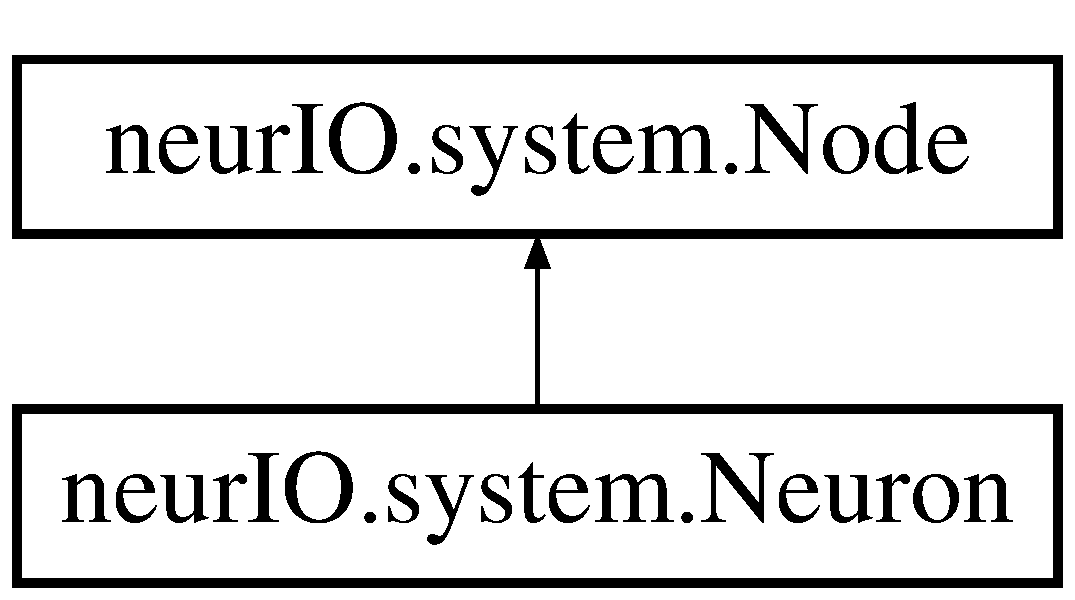
\includegraphics[height=2.000000cm]{classneur_i_o_1_1system_1_1_neuron}
\end{center}
\end{figure}
\subsection*{Classes}
\begin{DoxyCompactItemize}
\item 
class \hyperlink{classneur_i_o_1_1system_1_1_neuron_1_1_presets}{Presets}
\end{DoxyCompactItemize}
\subsection*{Public Member Functions}
\begin{DoxyCompactItemize}
\item 
\mbox{\Hypertarget{classneur_i_o_1_1system_1_1_neuron_af05fb9eac54b8f73ed831b3f1fd1f665}\label{classneur_i_o_1_1system_1_1_neuron_af05fb9eac54b8f73ed831b3f1fd1f665}} 
{\bfseries Neuron} (\hyperlink{classneur_i_o_1_1system_1_1_node}{Node}\mbox{[}$\,$\mbox{]} children, \hyperlink{classneur_i_o_1_1system_1_1_truth_table}{Truth\+Table} function)
\item 
\mbox{\Hypertarget{classneur_i_o_1_1system_1_1_neuron_afdfb793400c4507d3d94d07595e5f3f6}\label{classneur_i_o_1_1system_1_1_neuron_afdfb793400c4507d3d94d07595e5f3f6}} 
\hyperlink{classneur_i_o_1_1system_1_1_neuron}{Neuron} {\bfseries clone} (\hyperlink{classneur_i_o_1_1system_1_1_node}{Node}\mbox{[}$\,$\mbox{]} new\+Targets)
\item 
\mbox{\Hypertarget{classneur_i_o_1_1system_1_1_neuron_aa1ff6529c3a04fc5ecdaf41dd8a143cb}\label{classneur_i_o_1_1system_1_1_neuron_aa1ff6529c3a04fc5ecdaf41dd8a143cb}} 
boolean {\bfseries is\+Valid} ()
\item 
\mbox{\Hypertarget{classneur_i_o_1_1system_1_1_neuron_a7e2bfa3a562b6a26e3844d3285cbb669}\label{classneur_i_o_1_1system_1_1_neuron_a7e2bfa3a562b6a26e3844d3285cbb669}} 
boolean {\bfseries get\+Value} ()
\item 
\mbox{\Hypertarget{classneur_i_o_1_1system_1_1_neuron_a0adab143f0cbca556908f06d28cde838}\label{classneur_i_o_1_1system_1_1_neuron_a0adab143f0cbca556908f06d28cde838}} 
void {\bfseries reset\+Value} ()
\end{DoxyCompactItemize}
\subsection*{Additional Inherited Members}


The documentation for this class was generated from the following file\+:\begin{DoxyCompactItemize}
\item 
Neur\+I\+O/src/neur\+I\+O/system/Neuron.\+java\end{DoxyCompactItemize}

\hypertarget{classneur_i_o_1_1system_1_1_node}{}\section{neur\+I\+O.\+system.\+Node Class Reference}
\label{classneur_i_o_1_1system_1_1_node}\index{neur\+I\+O.\+system.\+Node@{neur\+I\+O.\+system.\+Node}}


Inheritance diagram for neur\+I\+O.\+system.\+Node\+:
% FIG 0
\subsection*{Public Member Functions}
\begin{DoxyCompactItemize}
\item 
\hyperlink{classneur_i_o_1_1system_1_1_node_a18dfd9e4acbf3ffbbd81870d2740254b}{Node} ()
\item 
\hyperlink{classneur_i_o_1_1system_1_1_node_a82de053582ee57d0ed239293a5b260ba}{Node} (boolean \hyperlink{classneur_i_o_1_1system_1_1_node_a2c6a229d3d2cbf1b313d8797b70e487a}{value})
\item 
boolean \hyperlink{classneur_i_o_1_1system_1_1_node_abcfb650e20f0e7b94dcdbcee0a92852c}{get\+Value} ()
\item 
void \hyperlink{classneur_i_o_1_1system_1_1_node_afd4bea06756a10a4dc05dc06afdcd459}{reset\+Value} ()
\end{DoxyCompactItemize}
\subsection*{Protected Attributes}
\begin{DoxyCompactItemize}
\item 
boolean \hyperlink{classneur_i_o_1_1system_1_1_node_a2c6a229d3d2cbf1b313d8797b70e487a}{value}
\end{DoxyCompactItemize}


\subsection{Detailed Description}
\subsection*{\hyperlink{classneur_i_o_1_1system_1_1_node}{Node} }

A lower level class that is used in columns and networks Allows for differentiation between Neurons(computational nodes), Inputs (constant nodes), and Outputs (resultant nodes) 

Definition at line 14 of file Node.\+java.



\subsection{Constructor \& Destructor Documentation}
\mbox{\Hypertarget{classneur_i_o_1_1system_1_1_node_a18dfd9e4acbf3ffbbd81870d2740254b}\label{classneur_i_o_1_1system_1_1_node_a18dfd9e4acbf3ffbbd81870d2740254b}} 
\index{neur\+I\+O\+::system\+::\+Node@{neur\+I\+O\+::system\+::\+Node}!Node@{Node}}
\index{Node@{Node}!neur\+I\+O\+::system\+::\+Node@{neur\+I\+O\+::system\+::\+Node}}
\subsubsection{\texorpdfstring{Node()}{Node()}\hspace{0.1cm}{\footnotesize\ttfamily [1/2]}}
{\footnotesize\ttfamily neur\+I\+O.\+system.\+Node.\+Node (\begin{DoxyParamCaption}{ }\end{DoxyParamCaption})}



Definition at line 17 of file Node.\+java.

\mbox{\Hypertarget{classneur_i_o_1_1system_1_1_node_a82de053582ee57d0ed239293a5b260ba}\label{classneur_i_o_1_1system_1_1_node_a82de053582ee57d0ed239293a5b260ba}} 
\index{neur\+I\+O\+::system\+::\+Node@{neur\+I\+O\+::system\+::\+Node}!Node@{Node}}
\index{Node@{Node}!neur\+I\+O\+::system\+::\+Node@{neur\+I\+O\+::system\+::\+Node}}
\subsubsection{\texorpdfstring{Node()}{Node()}\hspace{0.1cm}{\footnotesize\ttfamily [2/2]}}
{\footnotesize\ttfamily neur\+I\+O.\+system.\+Node.\+Node (\begin{DoxyParamCaption}\item[{boolean}]{value }\end{DoxyParamCaption})}



Definition at line 19 of file Node.\+java.



\subsection{Member Function Documentation}
\mbox{\Hypertarget{classneur_i_o_1_1system_1_1_node_abcfb650e20f0e7b94dcdbcee0a92852c}\label{classneur_i_o_1_1system_1_1_node_abcfb650e20f0e7b94dcdbcee0a92852c}} 
\index{neur\+I\+O\+::system\+::\+Node@{neur\+I\+O\+::system\+::\+Node}!get\+Value@{get\+Value}}
\index{get\+Value@{get\+Value}!neur\+I\+O\+::system\+::\+Node@{neur\+I\+O\+::system\+::\+Node}}
\subsubsection{\texorpdfstring{get\+Value()}{getValue()}}
{\footnotesize\ttfamily boolean neur\+I\+O.\+system.\+Node.\+get\+Value (\begin{DoxyParamCaption}{ }\end{DoxyParamCaption})}



Definition at line 23 of file Node.\+java.

\mbox{\Hypertarget{classneur_i_o_1_1system_1_1_node_afd4bea06756a10a4dc05dc06afdcd459}\label{classneur_i_o_1_1system_1_1_node_afd4bea06756a10a4dc05dc06afdcd459}} 
\index{neur\+I\+O\+::system\+::\+Node@{neur\+I\+O\+::system\+::\+Node}!reset\+Value@{reset\+Value}}
\index{reset\+Value@{reset\+Value}!neur\+I\+O\+::system\+::\+Node@{neur\+I\+O\+::system\+::\+Node}}
\subsubsection{\texorpdfstring{reset\+Value()}{resetValue()}}
{\footnotesize\ttfamily void neur\+I\+O.\+system.\+Node.\+reset\+Value (\begin{DoxyParamCaption}{ }\end{DoxyParamCaption})}



Definition at line 26 of file Node.\+java.



\subsection{Member Data Documentation}
\mbox{\Hypertarget{classneur_i_o_1_1system_1_1_node_a2c6a229d3d2cbf1b313d8797b70e487a}\label{classneur_i_o_1_1system_1_1_node_a2c6a229d3d2cbf1b313d8797b70e487a}} 
\index{neur\+I\+O\+::system\+::\+Node@{neur\+I\+O\+::system\+::\+Node}!value@{value}}
\index{value@{value}!neur\+I\+O\+::system\+::\+Node@{neur\+I\+O\+::system\+::\+Node}}
\subsubsection{\texorpdfstring{value}{value}}
{\footnotesize\ttfamily boolean neur\+I\+O.\+system.\+Node.\+value\hspace{0.3cm}{\ttfamily [protected]}}



Definition at line 15 of file Node.\+java.



The documentation for this class was generated from the following file\+:\begin{DoxyCompactItemize}
\item 
src/neur\+I\+O/system/\hyperlink{_node_8java}{Node.\+java}\end{DoxyCompactItemize}

\hypertarget{classneur_i_o_1_1system_1_1_output_node}{}\section{neur\+I\+O.\+system.\+Output\+Node Class Reference}
\label{classneur_i_o_1_1system_1_1_output_node}\index{neur\+I\+O.\+system.\+Output\+Node@{neur\+I\+O.\+system.\+Output\+Node}}
Inheritance diagram for neur\+I\+O.\+system.\+Output\+Node\+:\begin{figure}[H]
\begin{center}
\leavevmode
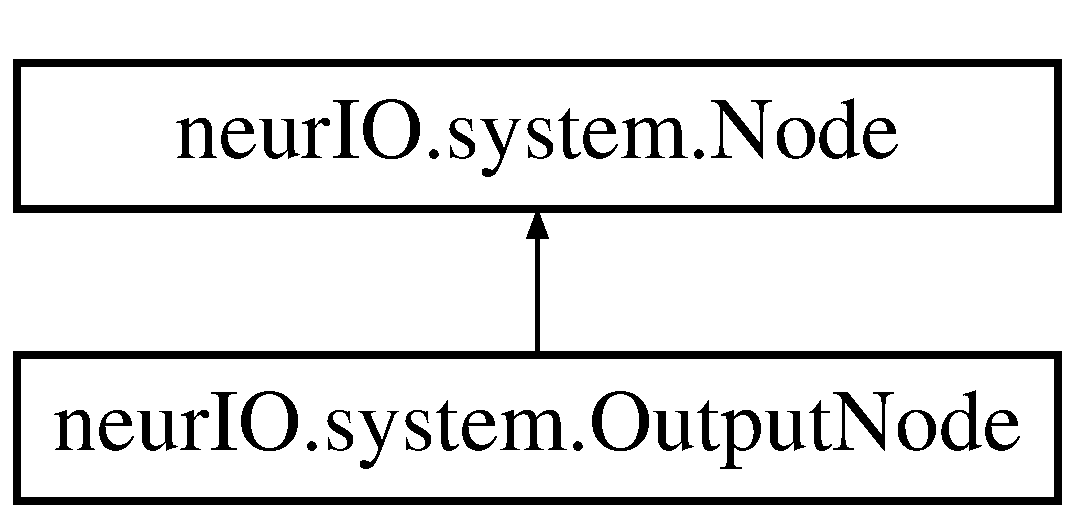
\includegraphics[height=2.000000cm]{classneur_i_o_1_1system_1_1_output_node}
\end{center}
\end{figure}
\subsection*{Public Member Functions}
\begin{DoxyCompactItemize}
\item 
\mbox{\Hypertarget{classneur_i_o_1_1system_1_1_output_node_ac4e8788594edf3352bb2037b7e505816}\label{classneur_i_o_1_1system_1_1_output_node_ac4e8788594edf3352bb2037b7e505816}} 
{\bfseries Output\+Node} (\hyperlink{classneur_i_o_1_1system_1_1_node}{Node} result)
\item 
\mbox{\Hypertarget{classneur_i_o_1_1system_1_1_output_node_ae5d244e5bb2168f66acbca5854fc614c}\label{classneur_i_o_1_1system_1_1_output_node_ae5d244e5bb2168f66acbca5854fc614c}} 
boolean {\bfseries get\+Value} ()
\end{DoxyCompactItemize}
\subsection*{Static Public Member Functions}
\begin{DoxyCompactItemize}
\item 
\mbox{\Hypertarget{classneur_i_o_1_1system_1_1_output_node_a7573728315335709ca81071b797f62b8}\label{classneur_i_o_1_1system_1_1_output_node_a7573728315335709ca81071b797f62b8}} 
static \hyperlink{classneur_i_o_1_1system_1_1_output_node}{Output\+Node} \mbox{[}$\,$\mbox{]} {\bfseries make\+Output\+Nodes} (Node...\+nodes)
\end{DoxyCompactItemize}
\subsection*{Additional Inherited Members}


The documentation for this class was generated from the following file\+:\begin{DoxyCompactItemize}
\item 
Neur\+I\+O/src/neur\+I\+O/system/Output\+Node.\+java\end{DoxyCompactItemize}

\hypertarget{classneur_i_o_1_1_start}{}\section{neur\+I\+O.\+Start Class Reference}
\label{classneur_i_o_1_1_start}\index{neur\+I\+O.\+Start@{neur\+I\+O.\+Start}}
\subsection*{Static Public Member Functions}
\begin{DoxyCompactItemize}
\item 
static void \hyperlink{classneur_i_o_1_1_start_aef3f6b2b34c677ae10ff69b507a2d4b4}{main} (String\mbox{[}$\,$\mbox{]} args)
\item 
static void \hyperlink{classneur_i_o_1_1_start_ae057e60dad95a9bd37e41c860cae2fab}{print\+Help} ()
\end{DoxyCompactItemize}
\subsection*{Static Private Member Functions}
\begin{DoxyCompactItemize}
\item 
static void \hyperlink{classneur_i_o_1_1_start_a2e18a32a484aa296caae592b4c8b9acd}{print\+Col\+Test} ()
\item 
static void \hyperlink{classneur_i_o_1_1_start_aedb59a7fabe14787e4d792a87bb23c7b}{print\+Truth\+Test} ()
\item 
static void \hyperlink{classneur_i_o_1_1_start_ae0f93675889ad60b4c42b39a64e94910}{print\+Network\+Test} ()
\end{DoxyCompactItemize}


\subsection{Detailed Description}
\subsection*{\hyperlink{classneur_i_o_1_1_start}{Start} }

This is the main class to start tests, G\+UI, etc. 

\subsection{Member Function Documentation}
\mbox{\Hypertarget{classneur_i_o_1_1_start_aef3f6b2b34c677ae10ff69b507a2d4b4}\label{classneur_i_o_1_1_start_aef3f6b2b34c677ae10ff69b507a2d4b4}} 
\index{neur\+I\+O\+::\+Start@{neur\+I\+O\+::\+Start}!main@{main}}
\index{main@{main}!neur\+I\+O\+::\+Start@{neur\+I\+O\+::\+Start}}
\subsubsection{\texorpdfstring{main()}{main()}}
{\footnotesize\ttfamily static void neur\+I\+O.\+Start.\+main (\begin{DoxyParamCaption}\item[{String \mbox{[}$\,$\mbox{]}}]{args }\end{DoxyParamCaption})\hspace{0.3cm}{\ttfamily [static]}}

The main program used to start the G\+UI, do tests, etc. This is N\+OT for A\+PI usage. 
\begin{DoxyCode}
28                                            \{
29         Global.args = args;
30         \hyperlink{classneur_i_o_1_1_start_a2e18a32a484aa296caae592b4c8b9acd}{printColTest}();
31         \hyperlink{classneur_i_o_1_1_start_aedb59a7fabe14787e4d792a87bb23c7b}{printTruthTest}();
32         \hyperlink{classneur_i_o_1_1_start_ae057e60dad95a9bd37e41c860cae2fab}{printHelp}();
33         \hyperlink{classneur_i_o_1_1_start_ae0f93675889ad60b4c42b39a64e94910}{printNetworkTest}();
34         \textcolor{keywordflow}{switch}(args[0])\{
35             default : \hyperlink{classneur_i_o_1_1_start_ae057e60dad95a9bd37e41c860cae2fab}{printHelp}();
36         \}
37     \}
\end{DoxyCode}
\mbox{\Hypertarget{classneur_i_o_1_1_start_a2e18a32a484aa296caae592b4c8b9acd}\label{classneur_i_o_1_1_start_a2e18a32a484aa296caae592b4c8b9acd}} 
\index{neur\+I\+O\+::\+Start@{neur\+I\+O\+::\+Start}!print\+Col\+Test@{print\+Col\+Test}}
\index{print\+Col\+Test@{print\+Col\+Test}!neur\+I\+O\+::\+Start@{neur\+I\+O\+::\+Start}}
\subsubsection{\texorpdfstring{print\+Col\+Test()}{printColTest()}}
{\footnotesize\ttfamily static void neur\+I\+O.\+Start.\+print\+Col\+Test (\begin{DoxyParamCaption}{ }\end{DoxyParamCaption})\hspace{0.3cm}{\ttfamily [static]}, {\ttfamily [private]}}

Tests the naming system of Columns. This is in excel (A-\/Z,A\+A-\/\+ZZ, etc) 
\begin{DoxyCode}
55                                        \{
56         \textcolor{keywordflow}{for}(\textcolor{keywordtype}{int} i = 0; i < 27; i++) \{
57             System.out.println(Truth.colIndexName(i));
58         \}
59     \}
\end{DoxyCode}
\mbox{\Hypertarget{classneur_i_o_1_1_start_ae057e60dad95a9bd37e41c860cae2fab}\label{classneur_i_o_1_1_start_ae057e60dad95a9bd37e41c860cae2fab}} 
\index{neur\+I\+O\+::\+Start@{neur\+I\+O\+::\+Start}!print\+Help@{print\+Help}}
\index{print\+Help@{print\+Help}!neur\+I\+O\+::\+Start@{neur\+I\+O\+::\+Start}}
\subsubsection{\texorpdfstring{print\+Help()}{printHelp()}}
{\footnotesize\ttfamily static void neur\+I\+O.\+Start.\+print\+Help (\begin{DoxyParamCaption}{ }\end{DoxyParamCaption})\hspace{0.3cm}{\ttfamily [static]}}

Doesn\textquotesingle{}t actually print any help at the moment...

will eventually print out a command line help form 
\begin{DoxyCode}
44                                   \{
45         System.out.println(\textcolor{stringliteral}{"NEURIO 2017 Brice Johnson"});
46         System.out.println(\textcolor{stringliteral}{"-----------------------------"});
47         System.out.println(\textcolor{stringliteral}{"           OPTIONS           "});
48         System.out.println(\textcolor{stringliteral}{"-----------------------------"});
49     \}
\end{DoxyCode}
\mbox{\Hypertarget{classneur_i_o_1_1_start_ae0f93675889ad60b4c42b39a64e94910}\label{classneur_i_o_1_1_start_ae0f93675889ad60b4c42b39a64e94910}} 
\index{neur\+I\+O\+::\+Start@{neur\+I\+O\+::\+Start}!print\+Network\+Test@{print\+Network\+Test}}
\index{print\+Network\+Test@{print\+Network\+Test}!neur\+I\+O\+::\+Start@{neur\+I\+O\+::\+Start}}
\subsubsection{\texorpdfstring{print\+Network\+Test()}{printNetworkTest()}}
{\footnotesize\ttfamily static void neur\+I\+O.\+Start.\+print\+Network\+Test (\begin{DoxyParamCaption}{ }\end{DoxyParamCaption})\hspace{0.3cm}{\ttfamily [static]}, {\ttfamily [private]}}

Prints out the result of a summing network which sums one byte at a time 
\begin{DoxyCode}
73                                           \{
74         \textcolor{keywordtype}{boolean}[] xor = \{\textcolor{keyword}{false},\textcolor{keyword}{true},\textcolor{keyword}{true},\textcolor{keyword}{false}\};
75         \textcolor{keywordtype}{boolean}[] and = \{\textcolor{keyword}{false},\textcolor{keyword}{false},\textcolor{keyword}{false},\textcolor{keyword}{true}\};
76         \textcolor{keywordtype}{boolean}[] sum = \{\textcolor{keyword}{false},\textcolor{keyword}{true},\textcolor{keyword}{true},\textcolor{keyword}{false},\textcolor{keyword}{true},\textcolor{keyword}{false},\textcolor{keyword}{false},\textcolor{keyword}{true}\};
77         \textcolor{keywordtype}{boolean}[] car = \{\textcolor{keyword}{false},\textcolor{keyword}{false},\textcolor{keyword}{false},\textcolor{keyword}{true},\textcolor{keyword}{false},\textcolor{keyword}{true},\textcolor{keyword}{true},\textcolor{keyword}{true}\};
78         
79         Network eightBitAdder = \textcolor{keyword}{new} Network(8,2);
80         BitInput A1 = \textcolor{keyword}{new} BitInput(\textcolor{keyword}{false}),
81         A2 = \textcolor{keyword}{new} BitInput(\textcolor{keyword}{false}),
82         A3 = \textcolor{keyword}{new} BitInput(\textcolor{keyword}{false}),
83         A4 = \textcolor{keyword}{new} BitInput(\textcolor{keyword}{false}),
84         A5 = \textcolor{keyword}{new} BitInput(\textcolor{keyword}{false}),
85         A6 = \textcolor{keyword}{new} BitInput(\textcolor{keyword}{false}),
86         A7 = \textcolor{keyword}{new} BitInput(\textcolor{keyword}{false}),
87         A8 = \textcolor{keyword}{new} BitInput(\textcolor{keyword}{false}),
88         B1 = \textcolor{keyword}{new} BitInput(\textcolor{keyword}{false}),
89         B2 = \textcolor{keyword}{new} BitInput(\textcolor{keyword}{false}),
90         B3 = \textcolor{keyword}{new} BitInput(\textcolor{keyword}{false}),
91         B4 = \textcolor{keyword}{new} BitInput(\textcolor{keyword}{false}),
92         B5 = \textcolor{keyword}{new} BitInput(\textcolor{keyword}{false}),
93         B6 = \textcolor{keyword}{new} BitInput(\textcolor{keyword}{false}),
94         B7 = \textcolor{keyword}{new} BitInput(\textcolor{keyword}{false}),
95         B8 = \textcolor{keyword}{new} BitInput(\textcolor{keyword}{false});
96         BitInput[] num1 = \{A1,A2,A3,A4,A5,A6,A7,A8\};
97         BitInput[] num2 = \{B1,B2,B3,B4,B5,B6,B7,B8\};
98         BitInput[] nums = \{A1,A2,A3,A4,A5,A6,A7,A8,B1,B2,B3,B4,B5,B6,B7,B8\};
99         BitInputSet bus1 = \textcolor{keyword}{new} BitInputSet(num1);
100         BitInputSet bus2 = \textcolor{keyword}{new} BitInputSet(num2);
101         
102         Column in = \textcolor{keyword}{new} Column(nums);
103         
104         eightBitAdder.input = in;
105         
106         bus1.numToInput(234);
107         bus2.numToInput(154);
108         
109         Node[] bitIns1 = \{A1,B1\};  \textcolor{comment}{//Add the first bit of numbers A and B together.}
110         Neuron sum1= \textcolor{keyword}{new} Neuron(bitIns1, \textcolor{keyword}{new} TruthTable(xor)); \textcolor{comment}{//Get the sum of the bits}
111         Neuron car1= \textcolor{keyword}{new} Neuron(bitIns1, \textcolor{keyword}{new} TruthTable(and)); \textcolor{comment}{//Get the carry of the bits}
112         Column c1 = (\textcolor{keyword}{new} Column(sum1,car1)); \textcolor{comment}{// Make into a function}
113         eightBitAdder.addColumn(c1);\textcolor{comment}{// Add to a network}
114         Node[] bitIns2 = \{A2,B2,car1\};\textcolor{comment}{//Add the last carry, and the second bits together.}
115         Neuron sum2 = \textcolor{keyword}{new} Neuron(bitIns2,\textcolor{keyword}{new} TruthTable(sum));\textcolor{comment}{// Different truth tables are used for 3
       bits.}
116         Neuron car2 = \textcolor{keyword}{new} Neuron(bitIns2,\textcolor{keyword}{new} TruthTable(car));
117         Column c2 = (\textcolor{keyword}{new} Column(sum2,car2));
118         eightBitAdder.addColumn(c2);
119         Node[] bitIns3 = \{A3,B3,car2\};
120         Neuron sum3 = \textcolor{keyword}{new} Neuron(bitIns3,\textcolor{keyword}{new} TruthTable(sum));
121         Neuron car3 = \textcolor{keyword}{new} Neuron(bitIns3,\textcolor{keyword}{new} TruthTable(car));
122         Column c3 = (\textcolor{keyword}{new} Column(sum3,car3));
123         eightBitAdder.addColumn(c3);
124         Node[] bitIns4 = \{A4,B4,car3\};
125         Neuron sum4 = \textcolor{keyword}{new} Neuron(bitIns4,\textcolor{keyword}{new} TruthTable(sum));
126         Neuron car4 = \textcolor{keyword}{new} Neuron(bitIns4,\textcolor{keyword}{new} TruthTable(car));
127         Column c4 = (\textcolor{keyword}{new} Column(sum4,car4));
128         eightBitAdder.addColumn(c4);
129         Node[] bitIns5 = \{A5,B5,car4\};
130         Neuron sum5 = \textcolor{keyword}{new} Neuron(bitIns5,\textcolor{keyword}{new} TruthTable(sum));
131         Neuron car5 = \textcolor{keyword}{new} Neuron(bitIns5,\textcolor{keyword}{new} TruthTable(car));
132         Column c5 = (\textcolor{keyword}{new} Column(sum5,car5));
133         eightBitAdder.addColumn(c5);
134         Node[] bitIns6 = \{A6,B6,car5\};
135         Neuron sum6 = \textcolor{keyword}{new} Neuron(bitIns6,\textcolor{keyword}{new} TruthTable(sum));
136         Neuron car6 = \textcolor{keyword}{new} Neuron(bitIns6,\textcolor{keyword}{new} TruthTable(car));
137         Column c6 = (\textcolor{keyword}{new} Column(sum6,car6));
138         eightBitAdder.addColumn(c6);
139         Node[] bitIns7 = \{A7,B7,car6\};
140         Neuron sum7 = \textcolor{keyword}{new} Neuron(bitIns7,\textcolor{keyword}{new} TruthTable(sum));
141         Neuron car7 = \textcolor{keyword}{new} Neuron(bitIns7,\textcolor{keyword}{new} TruthTable(car));
142         Column c7 = (\textcolor{keyword}{new} Column(sum7,car7));
143         eightBitAdder.addColumn(c7);
144         Node[] bitIns8 = \{A8,B8,car7\};
145         Neuron sum8 = \textcolor{keyword}{new} Neuron(bitIns8,\textcolor{keyword}{new} TruthTable(sum));
146         Neuron car8 = \textcolor{keyword}{new} Neuron(bitIns8,\textcolor{keyword}{new} TruthTable(car));
147         Column c8 = (\textcolor{keyword}{new} Column(sum8,car8));
148         eightBitAdder.addColumn(c8);
149         OutputNode[] outputNodes = OutputNode.makeOutputNodes(sum1,sum2,sum3,sum4,sum5,sum6,sum7,sum8,car8)
      ;
150         Column outputColumn = \textcolor{keyword}{new} Column(outputNodes);
151         eightBitAdder.output = outputColumn;
152         
153         \textcolor{keywordtype}{int} result = 0;
154         \textcolor{keywordflow}{for}(\textcolor{keywordtype}{int} i = 0; i < outputNodes.length; i++)\{
155             System.out.println(outputNodes[i].getValue());
156             result +=(outputNodes[i].getValue()?1:0)<<i;
157         \}
158         
159         System.out.println(result);
160         
161     \}
\end{DoxyCode}
\mbox{\Hypertarget{classneur_i_o_1_1_start_aedb59a7fabe14787e4d792a87bb23c7b}\label{classneur_i_o_1_1_start_aedb59a7fabe14787e4d792a87bb23c7b}} 
\index{neur\+I\+O\+::\+Start@{neur\+I\+O\+::\+Start}!print\+Truth\+Test@{print\+Truth\+Test}}
\index{print\+Truth\+Test@{print\+Truth\+Test}!neur\+I\+O\+::\+Start@{neur\+I\+O\+::\+Start}}
\subsubsection{\texorpdfstring{print\+Truth\+Test()}{printTruthTest()}}
{\footnotesize\ttfamily static void neur\+I\+O.\+Start.\+print\+Truth\+Test (\begin{DoxyParamCaption}{ }\end{DoxyParamCaption})\hspace{0.3cm}{\ttfamily [static]}, {\ttfamily [private]}}

Prints a truth table using the To\+String test. 
\begin{DoxyCode}
64                                         \{
65         \textcolor{keywordtype}{boolean}[] conditions = \{\textcolor{keyword}{false}, \textcolor{keyword}{false}, \textcolor{keyword}{true}\};
66         Truth truth = \textcolor{keyword}{new} Truth(conditions, \textcolor{keyword}{true});
67         System.out.println(truth.toString());
68     \}
\end{DoxyCode}


The documentation for this class was generated from the following file\+:\begin{DoxyCompactItemize}
\item 
Neur\+I\+O/src/neur\+I\+O/Start.\+java\end{DoxyCompactItemize}

\hypertarget{classneur_i_o_1_1system_1_1_truth}{}\section{neur\+I\+O.\+system.\+Truth Class Reference}
\label{classneur_i_o_1_1system_1_1_truth}\index{neur\+I\+O.\+system.\+Truth@{neur\+I\+O.\+system.\+Truth}}
\subsection*{Public Member Functions}
\begin{DoxyCompactItemize}
\item 
\mbox{\Hypertarget{classneur_i_o_1_1system_1_1_truth_a097cc75403bc8483160fb5668f0fd039}\label{classneur_i_o_1_1system_1_1_truth_a097cc75403bc8483160fb5668f0fd039}} 
{\bfseries Truth} (int width)
\item 
\mbox{\Hypertarget{classneur_i_o_1_1system_1_1_truth_a448eb40dceba7515b95ad0c408ac9dc0}\label{classneur_i_o_1_1system_1_1_truth_a448eb40dceba7515b95ad0c408ac9dc0}} 
{\bfseries Truth} (String name, int width, boolean result)
\item 
\mbox{\Hypertarget{classneur_i_o_1_1system_1_1_truth_a8241dbb4e9d35b2d8eb95676752a2b3e}\label{classneur_i_o_1_1system_1_1_truth_a8241dbb4e9d35b2d8eb95676752a2b3e}} 
{\bfseries Truth} (int width, boolean result)
\item 
\mbox{\Hypertarget{classneur_i_o_1_1system_1_1_truth_ab07669c710b191e33cc173e0facb9c5c}\label{classneur_i_o_1_1system_1_1_truth_ab07669c710b191e33cc173e0facb9c5c}} 
{\bfseries Truth} (boolean\mbox{[}$\,$\mbox{]} conditions, boolean result)
\item 
\mbox{\Hypertarget{classneur_i_o_1_1system_1_1_truth_af87a339fee0afc3c42f31770474d8b41}\label{classneur_i_o_1_1system_1_1_truth_af87a339fee0afc3c42f31770474d8b41}} 
{\bfseries Truth} (String name, boolean\mbox{[}$\,$\mbox{]} conditions, boolean result)
\item 
\mbox{\Hypertarget{classneur_i_o_1_1system_1_1_truth_a842f96b6b8887a8c0efaa6d2b9f1a7c4}\label{classneur_i_o_1_1system_1_1_truth_a842f96b6b8887a8c0efaa6d2b9f1a7c4}} 
int {\bfseries get\+Width} ()
\item 
\mbox{\Hypertarget{classneur_i_o_1_1system_1_1_truth_a7f4d8c214884a035c30e6eb9accb4eb3}\label{classneur_i_o_1_1system_1_1_truth_a7f4d8c214884a035c30e6eb9accb4eb3}} 
\hyperlink{classneur_i_o_1_1system_1_1_truth}{Truth} {\bfseries add\+Param} (boolean param)
\item 
\mbox{\Hypertarget{classneur_i_o_1_1system_1_1_truth_ac7f532c2a20156db2b85b799730ee959}\label{classneur_i_o_1_1system_1_1_truth_ac7f532c2a20156db2b85b799730ee959}} 
String {\bfseries to\+String} ()
\end{DoxyCompactItemize}
\subsection*{Static Public Member Functions}
\begin{DoxyCompactItemize}
\item 
\mbox{\Hypertarget{classneur_i_o_1_1system_1_1_truth_a111599cd27bfb1e906cad589313c02d7}\label{classneur_i_o_1_1system_1_1_truth_a111599cd27bfb1e906cad589313c02d7}} 
static String {\bfseries col\+Index\+Name} (int index)
\end{DoxyCompactItemize}
\subsection*{Public Attributes}
\begin{DoxyCompactItemize}
\item 
\mbox{\Hypertarget{classneur_i_o_1_1system_1_1_truth_a73e0e02b8591832131d0c26d1f88dea2}\label{classneur_i_o_1_1system_1_1_truth_a73e0e02b8591832131d0c26d1f88dea2}} 
String {\bfseries name} = \char`\"{}\char`\"{}
\end{DoxyCompactItemize}
\subsection*{Private Member Functions}
\begin{DoxyCompactItemize}
\item 
\mbox{\Hypertarget{classneur_i_o_1_1system_1_1_truth_ab87b56891179c3a4409c0b953867453a}\label{classneur_i_o_1_1system_1_1_truth_ab87b56891179c3a4409c0b953867453a}} 
String {\bfseries generate\+String\+Truth} ()
\item 
\mbox{\Hypertarget{classneur_i_o_1_1system_1_1_truth_a36c7d311f47af72a2fe8d4689de4d9c1}\label{classneur_i_o_1_1system_1_1_truth_a36c7d311f47af72a2fe8d4689de4d9c1}} 
String {\bfseries generate\+String\+Header} ()
\end{DoxyCompactItemize}


The documentation for this class was generated from the following file\+:\begin{DoxyCompactItemize}
\item 
Neur\+I\+O/src/neur\+I\+O/system/Truth.\+java\end{DoxyCompactItemize}

\hypertarget{classneur_i_o_1_1system_1_1_truth_table}{}\section{neur\+I\+O.\+system.\+Truth\+Table Class Reference}
\label{classneur_i_o_1_1system_1_1_truth_table}\index{neur\+I\+O.\+system.\+Truth\+Table@{neur\+I\+O.\+system.\+Truth\+Table}}


Collaboration diagram for neur\+I\+O.\+system.\+Truth\+Table\+:
% FIG 0
\subsection*{Public Member Functions}
\begin{DoxyCompactItemize}
\item 
\hyperlink{classneur_i_o_1_1system_1_1_truth_table_a9a4e5d68d6f275a51c7af28c5e4f11c2}{Truth\+Table} (boolean\mbox{[}$\,$\mbox{]} results)
\item 
boolean \hyperlink{classneur_i_o_1_1system_1_1_truth_table_a47bb5f7ba445758e1b892e079c501212}{get\+Result} (boolean\mbox{[}$\,$\mbox{]} truth)
\item 
boolean \hyperlink{classneur_i_o_1_1system_1_1_truth_table_a0932bf77d2e3e05e0a317f8003e67e53}{is\+Complete} ()
\item 
\hyperlink{classneur_i_o_1_1system_1_1_truth}{Truth} \hyperlink{classneur_i_o_1_1system_1_1_truth_table_a855f811de0244489c48772a0511b48ce}{get\+Truth} (boolean\mbox{[}$\,$\mbox{]} truth)
\end{DoxyCompactItemize}
\subsection*{Static Public Member Functions}
\begin{DoxyCompactItemize}
\item 
static \hyperlink{classneur_i_o_1_1system_1_1_truth}{Truth} \mbox{[}$\,$\mbox{]} \hyperlink{classneur_i_o_1_1system_1_1_truth_table_a1146ea2f3e41f379b920947a2ad840d8}{make\+Truths} (boolean\mbox{[}$\,$\mbox{]} results, int \hyperlink{classneur_i_o_1_1system_1_1_truth_table_a71a416200e01a326bad83c9509cca9f1}{width})
\end{DoxyCompactItemize}
\subsection*{Public Attributes}
\begin{DoxyCompactItemize}
\item 
\hyperlink{classneur_i_o_1_1system_1_1_truth}{Truth} \mbox{[}$\,$\mbox{]} \hyperlink{classneur_i_o_1_1system_1_1_truth_table_aa8cdabf1eb334fc405d50b9249e42ae4}{truths}
\item 
int \hyperlink{classneur_i_o_1_1system_1_1_truth_table_a71a416200e01a326bad83c9509cca9f1}{width}
\end{DoxyCompactItemize}


\subsection{Detailed Description}


Definition at line 8 of file Truth\+Table.\+java.



\subsection{Constructor \& Destructor Documentation}
\mbox{\Hypertarget{classneur_i_o_1_1system_1_1_truth_table_a9a4e5d68d6f275a51c7af28c5e4f11c2}\label{classneur_i_o_1_1system_1_1_truth_table_a9a4e5d68d6f275a51c7af28c5e4f11c2}} 
\index{neur\+I\+O\+::system\+::\+Truth\+Table@{neur\+I\+O\+::system\+::\+Truth\+Table}!Truth\+Table@{Truth\+Table}}
\index{Truth\+Table@{Truth\+Table}!neur\+I\+O\+::system\+::\+Truth\+Table@{neur\+I\+O\+::system\+::\+Truth\+Table}}
\subsubsection{\texorpdfstring{Truth\+Table()}{TruthTable()}}
{\footnotesize\ttfamily neur\+I\+O.\+system.\+Truth\+Table.\+Truth\+Table (\begin{DoxyParamCaption}\item[{boolean \mbox{[}$\,$\mbox{]}}]{results }\end{DoxyParamCaption})}



Definition at line 18 of file Truth\+Table.\+java.



\subsection{Member Function Documentation}
\mbox{\Hypertarget{classneur_i_o_1_1system_1_1_truth_table_a47bb5f7ba445758e1b892e079c501212}\label{classneur_i_o_1_1system_1_1_truth_table_a47bb5f7ba445758e1b892e079c501212}} 
\index{neur\+I\+O\+::system\+::\+Truth\+Table@{neur\+I\+O\+::system\+::\+Truth\+Table}!get\+Result@{get\+Result}}
\index{get\+Result@{get\+Result}!neur\+I\+O\+::system\+::\+Truth\+Table@{neur\+I\+O\+::system\+::\+Truth\+Table}}
\subsubsection{\texorpdfstring{get\+Result()}{getResult()}}
{\footnotesize\ttfamily boolean neur\+I\+O.\+system.\+Truth\+Table.\+get\+Result (\begin{DoxyParamCaption}\item[{boolean \mbox{[}$\,$\mbox{]}}]{truth }\end{DoxyParamCaption})}



Definition at line 36 of file Truth\+Table.\+java.

\mbox{\Hypertarget{classneur_i_o_1_1system_1_1_truth_table_a855f811de0244489c48772a0511b48ce}\label{classneur_i_o_1_1system_1_1_truth_table_a855f811de0244489c48772a0511b48ce}} 
\index{neur\+I\+O\+::system\+::\+Truth\+Table@{neur\+I\+O\+::system\+::\+Truth\+Table}!get\+Truth@{get\+Truth}}
\index{get\+Truth@{get\+Truth}!neur\+I\+O\+::system\+::\+Truth\+Table@{neur\+I\+O\+::system\+::\+Truth\+Table}}
\subsubsection{\texorpdfstring{get\+Truth()}{getTruth()}}
{\footnotesize\ttfamily \hyperlink{classneur_i_o_1_1system_1_1_truth}{Truth} neur\+I\+O.\+system.\+Truth\+Table.\+get\+Truth (\begin{DoxyParamCaption}\item[{boolean \mbox{[}$\,$\mbox{]}}]{truth }\end{DoxyParamCaption})}



Definition at line 52 of file Truth\+Table.\+java.

\mbox{\Hypertarget{classneur_i_o_1_1system_1_1_truth_table_a0932bf77d2e3e05e0a317f8003e67e53}\label{classneur_i_o_1_1system_1_1_truth_table_a0932bf77d2e3e05e0a317f8003e67e53}} 
\index{neur\+I\+O\+::system\+::\+Truth\+Table@{neur\+I\+O\+::system\+::\+Truth\+Table}!is\+Complete@{is\+Complete}}
\index{is\+Complete@{is\+Complete}!neur\+I\+O\+::system\+::\+Truth\+Table@{neur\+I\+O\+::system\+::\+Truth\+Table}}
\subsubsection{\texorpdfstring{is\+Complete()}{isComplete()}}
{\footnotesize\ttfamily boolean neur\+I\+O.\+system.\+Truth\+Table.\+is\+Complete (\begin{DoxyParamCaption}{ }\end{DoxyParamCaption})}



Definition at line 48 of file Truth\+Table.\+java.

\mbox{\Hypertarget{classneur_i_o_1_1system_1_1_truth_table_a1146ea2f3e41f379b920947a2ad840d8}\label{classneur_i_o_1_1system_1_1_truth_table_a1146ea2f3e41f379b920947a2ad840d8}} 
\index{neur\+I\+O\+::system\+::\+Truth\+Table@{neur\+I\+O\+::system\+::\+Truth\+Table}!make\+Truths@{make\+Truths}}
\index{make\+Truths@{make\+Truths}!neur\+I\+O\+::system\+::\+Truth\+Table@{neur\+I\+O\+::system\+::\+Truth\+Table}}
\subsubsection{\texorpdfstring{make\+Truths()}{makeTruths()}}
{\footnotesize\ttfamily static \hyperlink{classneur_i_o_1_1system_1_1_truth}{Truth} \mbox{[}$\,$\mbox{]} neur\+I\+O.\+system.\+Truth\+Table.\+make\+Truths (\begin{DoxyParamCaption}\item[{boolean \mbox{[}$\,$\mbox{]}}]{results,  }\item[{int}]{width }\end{DoxyParamCaption})\hspace{0.3cm}{\ttfamily [static]}}



Definition at line 24 of file Truth\+Table.\+java.



\subsection{Member Data Documentation}
\mbox{\Hypertarget{classneur_i_o_1_1system_1_1_truth_table_aa8cdabf1eb334fc405d50b9249e42ae4}\label{classneur_i_o_1_1system_1_1_truth_table_aa8cdabf1eb334fc405d50b9249e42ae4}} 
\index{neur\+I\+O\+::system\+::\+Truth\+Table@{neur\+I\+O\+::system\+::\+Truth\+Table}!truths@{truths}}
\index{truths@{truths}!neur\+I\+O\+::system\+::\+Truth\+Table@{neur\+I\+O\+::system\+::\+Truth\+Table}}
\subsubsection{\texorpdfstring{truths}{truths}}
{\footnotesize\ttfamily \hyperlink{classneur_i_o_1_1system_1_1_truth}{Truth} \mbox{[}$\,$\mbox{]} neur\+I\+O.\+system.\+Truth\+Table.\+truths}

\subsection*{\hyperlink{classneur_i_o_1_1system_1_1_truth_table}{Truth\+Table} }

A truth table contains outputs for every combination of inputs of length n. The current configuration of this class allows for some inputs to be missing, making the table incomplete. 

Definition at line 15 of file Truth\+Table.\+java.

\mbox{\Hypertarget{classneur_i_o_1_1system_1_1_truth_table_a71a416200e01a326bad83c9509cca9f1}\label{classneur_i_o_1_1system_1_1_truth_table_a71a416200e01a326bad83c9509cca9f1}} 
\index{neur\+I\+O\+::system\+::\+Truth\+Table@{neur\+I\+O\+::system\+::\+Truth\+Table}!width@{width}}
\index{width@{width}!neur\+I\+O\+::system\+::\+Truth\+Table@{neur\+I\+O\+::system\+::\+Truth\+Table}}
\subsubsection{\texorpdfstring{width}{width}}
{\footnotesize\ttfamily int neur\+I\+O.\+system.\+Truth\+Table.\+width}



Definition at line 16 of file Truth\+Table.\+java.



The documentation for this class was generated from the following file\+:\begin{DoxyCompactItemize}
\item 
src/neur\+I\+O/system/\hyperlink{_truth_table_8java}{Truth\+Table.\+java}\end{DoxyCompactItemize}

\chapter{File Documentation}
\hypertarget{main_win_8java}{}\section{src/main\+Win.java File Reference}
\label{main_win_8java}\index{src/main\+Win.\+java@{src/main\+Win.\+java}}
\subsection*{Classes}
\begin{DoxyCompactItemize}
\item 
class \hyperlink{classmain_win}{main\+Win}
\end{DoxyCompactItemize}

\hypertarget{neur_i_o_2gui_2main_win_8java}{}\section{src/neur\+I\+O/gui/main\+Win.java File Reference}
\label{neur_i_o_2gui_2main_win_8java}\index{src/neur\+I\+O/gui/main\+Win.\+java@{src/neur\+I\+O/gui/main\+Win.\+java}}
\subsection*{Classes}
\begin{DoxyCompactItemize}
\item 
class \hyperlink{classneur_i_o_1_1gui_1_1main_win}{neur\+I\+O.\+gui.\+main\+Win}
\end{DoxyCompactItemize}
\subsection*{Packages}
\begin{DoxyCompactItemize}
\item 
package \hyperlink{namespaceneur_i_o_1_1gui}{neur\+I\+O.\+gui}
\end{DoxyCompactItemize}

\hypertarget{_bit_input_8java}{}\section{src/neur\+I\+O/data/bit\+Input/\+Bit\+Input.java File Reference}
\label{_bit_input_8java}\index{src/neur\+I\+O/data/bit\+Input/\+Bit\+Input.\+java@{src/neur\+I\+O/data/bit\+Input/\+Bit\+Input.\+java}}
\subsection*{Classes}
\begin{DoxyCompactItemize}
\item 
class \hyperlink{classneur_i_o_1_1data_1_1bit_input_1_1_bit_input}{neur\+I\+O.\+data.\+bit\+Input.\+Bit\+Input}
\end{DoxyCompactItemize}
\subsection*{Packages}
\begin{DoxyCompactItemize}
\item 
package \hyperlink{namespaceneur_i_o_1_1data_1_1bit_input}{neur\+I\+O.\+data.\+bit\+Input}
\end{DoxyCompactItemize}

\hypertarget{_bit_input_set_8java}{}\section{src/neur\+I\+O/data/bit\+Input/\+Bit\+Input\+Set.java File Reference}
\label{_bit_input_set_8java}\index{src/neur\+I\+O/data/bit\+Input/\+Bit\+Input\+Set.\+java@{src/neur\+I\+O/data/bit\+Input/\+Bit\+Input\+Set.\+java}}
\subsection*{Classes}
\begin{DoxyCompactItemize}
\item 
class \hyperlink{classneur_i_o_1_1data_1_1bit_input_1_1_bit_input_set}{neur\+I\+O.\+data.\+bit\+Input.\+Bit\+Input\+Set}
\end{DoxyCompactItemize}
\subsection*{Packages}
\begin{DoxyCompactItemize}
\item 
package \hyperlink{namespaceneur_i_o_1_1data_1_1bit_input}{neur\+I\+O.\+data.\+bit\+Input}
\end{DoxyCompactItemize}

\hypertarget{_bit_pagenator_8java}{}\section{src/neur\+I\+O/data/\+Bit\+Pagenator.java File Reference}
\label{_bit_pagenator_8java}\index{src/neur\+I\+O/data/\+Bit\+Pagenator.\+java@{src/neur\+I\+O/data/\+Bit\+Pagenator.\+java}}
\subsection*{Classes}
\begin{DoxyCompactItemize}
\item 
class \hyperlink{classneur_i_o_1_1data_1_1_bit_pagenator}{neur\+I\+O.\+data.\+Bit\+Pagenator}
\end{DoxyCompactItemize}
\subsection*{Packages}
\begin{DoxyCompactItemize}
\item 
package \hyperlink{namespaceneur_i_o_1_1data}{neur\+I\+O.\+data}
\end{DoxyCompactItemize}

\hypertarget{_bit_set_8java}{}\section{src/neur\+I\+O/data/\+Bit\+Set.java File Reference}
\label{_bit_set_8java}\index{src/neur\+I\+O/data/\+Bit\+Set.\+java@{src/neur\+I\+O/data/\+Bit\+Set.\+java}}
\subsection*{Classes}
\begin{DoxyCompactItemize}
\item 
class \hyperlink{classneur_i_o_1_1data_1_1_bit_set}{neur\+I\+O.\+data.\+Bit\+Set}
\end{DoxyCompactItemize}
\subsection*{Packages}
\begin{DoxyCompactItemize}
\item 
package \hyperlink{namespaceneur_i_o_1_1data}{neur\+I\+O.\+data}
\end{DoxyCompactItemize}

\hypertarget{_column_8java}{}\section{src/neur\+I\+O/engine/\+Column.java File Reference}
\label{_column_8java}\index{src/neur\+I\+O/engine/\+Column.\+java@{src/neur\+I\+O/engine/\+Column.\+java}}
\subsection*{Classes}
\begin{DoxyCompactItemize}
\item 
class \hyperlink{classneur_i_o_1_1engine_1_1_column}{neur\+I\+O.\+engine.\+Column}
\end{DoxyCompactItemize}
\subsection*{Packages}
\begin{DoxyCompactItemize}
\item 
package \hyperlink{namespaceneur_i_o_1_1engine}{neur\+I\+O.\+engine}
\end{DoxyCompactItemize}

\hypertarget{_network_8java}{}\section{src/neur\+I\+O/engine/\+Network.java File Reference}
\label{_network_8java}\index{src/neur\+I\+O/engine/\+Network.\+java@{src/neur\+I\+O/engine/\+Network.\+java}}
\subsection*{Classes}
\begin{DoxyCompactItemize}
\item 
class \hyperlink{classneur_i_o_1_1engine_1_1_network}{neur\+I\+O.\+engine.\+Network}
\end{DoxyCompactItemize}
\subsection*{Packages}
\begin{DoxyCompactItemize}
\item 
package \hyperlink{namespaceneur_i_o_1_1engine}{neur\+I\+O.\+engine}
\end{DoxyCompactItemize}

\hypertarget{_global_8java}{}\section{src/neur\+I\+O/\+Global.java File Reference}
\label{_global_8java}\index{src/neur\+I\+O/\+Global.\+java@{src/neur\+I\+O/\+Global.\+java}}
\subsection*{Classes}
\begin{DoxyCompactItemize}
\item 
class \hyperlink{classneur_i_o_1_1_global}{neur\+I\+O.\+Global}
\end{DoxyCompactItemize}
\subsection*{Packages}
\begin{DoxyCompactItemize}
\item 
package \hyperlink{namespaceneur_i_o}{neur\+IO}
\end{DoxyCompactItemize}

\hypertarget{_start_8java}{}\section{src/neur\+I\+O/\+Start.java File Reference}
\label{_start_8java}\index{src/neur\+I\+O/\+Start.\+java@{src/neur\+I\+O/\+Start.\+java}}
\subsection*{Classes}
\begin{DoxyCompactItemize}
\item 
class \hyperlink{classneur_i_o_1_1_start}{neur\+I\+O.\+Start}
\end{DoxyCompactItemize}
\subsection*{Packages}
\begin{DoxyCompactItemize}
\item 
package \hyperlink{namespaceneur_i_o}{neur\+IO}
\end{DoxyCompactItemize}

\hypertarget{_neuron_8java}{}\section{src/neur\+I\+O/system/\+Neuron.java File Reference}
\label{_neuron_8java}\index{src/neur\+I\+O/system/\+Neuron.\+java@{src/neur\+I\+O/system/\+Neuron.\+java}}
\subsection*{Classes}
\begin{DoxyCompactItemize}
\item 
class \hyperlink{classneur_i_o_1_1system_1_1_neuron}{neur\+I\+O.\+system.\+Neuron}
\item 
class {\bfseries neur\+I\+O.\+system.\+Neuron.\+Presets}
\end{DoxyCompactItemize}
\subsection*{Packages}
\begin{DoxyCompactItemize}
\item 
package \hyperlink{namespaceneur_i_o_1_1system}{neur\+I\+O.\+system}
\end{DoxyCompactItemize}

\hypertarget{_node_8java}{}\section{src/neur\+I\+O/system/\+Node.java File Reference}
\label{_node_8java}\index{src/neur\+I\+O/system/\+Node.\+java@{src/neur\+I\+O/system/\+Node.\+java}}
\subsection*{Classes}
\begin{DoxyCompactItemize}
\item 
class \hyperlink{classneur_i_o_1_1system_1_1_node}{neur\+I\+O.\+system.\+Node}
\end{DoxyCompactItemize}
\subsection*{Packages}
\begin{DoxyCompactItemize}
\item 
package \hyperlink{namespaceneur_i_o_1_1system}{neur\+I\+O.\+system}
\end{DoxyCompactItemize}

\hypertarget{_output_node_8java}{}\section{src/neur\+I\+O/system/\+Output\+Node.java File Reference}
\label{_output_node_8java}\index{src/neur\+I\+O/system/\+Output\+Node.\+java@{src/neur\+I\+O/system/\+Output\+Node.\+java}}
\subsection*{Classes}
\begin{DoxyCompactItemize}
\item 
class \hyperlink{classneur_i_o_1_1system_1_1_output_node}{neur\+I\+O.\+system.\+Output\+Node}
\end{DoxyCompactItemize}
\subsection*{Packages}
\begin{DoxyCompactItemize}
\item 
package \hyperlink{namespaceneur_i_o_1_1system}{neur\+I\+O.\+system}
\end{DoxyCompactItemize}

\hypertarget{_truth_8java}{}\section{src/neur\+I\+O/system/\+Truth.java File Reference}
\label{_truth_8java}\index{src/neur\+I\+O/system/\+Truth.\+java@{src/neur\+I\+O/system/\+Truth.\+java}}
\subsection*{Classes}
\begin{DoxyCompactItemize}
\item 
class \hyperlink{classneur_i_o_1_1system_1_1_truth}{neur\+I\+O.\+system.\+Truth}
\end{DoxyCompactItemize}
\subsection*{Packages}
\begin{DoxyCompactItemize}
\item 
package \hyperlink{namespaceneur_i_o_1_1system}{neur\+I\+O.\+system}
\end{DoxyCompactItemize}

\hypertarget{_truth_table_8java}{}\section{src/neur\+I\+O/system/\+Truth\+Table.java File Reference}
\label{_truth_table_8java}\index{src/neur\+I\+O/system/\+Truth\+Table.\+java@{src/neur\+I\+O/system/\+Truth\+Table.\+java}}
\subsection*{Classes}
\begin{DoxyCompactItemize}
\item 
class \hyperlink{classneur_i_o_1_1system_1_1_truth_table}{neur\+I\+O.\+system.\+Truth\+Table}
\end{DoxyCompactItemize}
\subsection*{Packages}
\begin{DoxyCompactItemize}
\item 
package \hyperlink{namespaceneur_i_o_1_1system}{neur\+I\+O.\+system}
\end{DoxyCompactItemize}

%--- End generated contents ---

% Index
\backmatter
\newpage
\phantomsection
\clearemptydoublepage
\addcontentsline{toc}{chapter}{Index}
\printindex

\end{document}
